\documentclass[a4paper]{article}
\usepackage{vntex}
%\usepackage[english,vietnam]{babel}
%\usepackage[utf8]{inputenc}

%\usepackage[utf8]{inputenc}
%\usepackage[francais]{babel}
\usepackage{a4wide,amssymb,epsfig,latexsym,multicol,array,hhline,fancyhdr}
\usepackage{booktabs}
\usepackage{amsmath}
\usepackage{lastpage}
\usepackage[lined,boxed,commentsnumbered]{algorithm2e}
\usepackage{enumerate}
\usepackage{color}
\usepackage{graphicx}							% Standard graphics package
\usepackage{array}
\usepackage{tabularx, caption}
\usepackage{multirow}
\usepackage[framemethod=tikz]{mdframed}% For highlighting paragraph backgrounds
\usepackage{multicol}
\usepackage{rotating}
\usepackage{graphics}
\usepackage[left=3cm,right=2cm,top=2cm,bottom=2cm]{geometry}
\usepackage{colortbl}
\usepackage{setspace}
\usepackage{epsfig}
\usepackage{tikz}
\usepackage{listings}
\usetikzlibrary{arrows,snakes,backgrounds}
\usepackage{hyperref}
\hypersetup{urlcolor=blue,linkcolor=black,citecolor=black,colorlinks=true}
\usepackage{float}
%\usepackage{pstcol} 								% PSTricks with the standard color package

\newtheorem{theorem}{{\bf Định lý}}
\newtheorem{property}{{\bf Tính chất}}
\newtheorem{proposition}{{\bf Mệnh đề}}
\newtheorem{corollary}[proposition]{{\bf Hệ quả}}
\newtheorem{lemma}[proposition]{{\bf Bổ đề}}

\everymath{\color{blue}}
%\usepackage{fancyhdr}
\setlength{\headheight}{40pt}
\pagestyle{fancy}
\fancyhead{} % clear all header fields
\fancyhead[L]{
 \begin{tabular}{rl}
    \begin{picture}(25,15)(0,0)
    \put(0,-8){
\includegraphics[width=8mm, height=8mm]{logoITSGUsmall.png}}
    %\put(0,-8){\epsfig{width=10mm,figure=hcmut.eps}}
   \end{picture}&
	%\includegraphics[width=8mm, height=8mm]{hcmut.png} & %
	\begin{tabular}{l}
		\textbf{\bf \ttfamily Trường Đại học Sài Gòn}\\
		\textbf{\bf \ttfamily Khoa Công Nghệ Thông Tin}
	\end{tabular} 	
 \end{tabular}
}
\fancyhead[R]{
	\begin{tabular}{l}
		\tiny \bf \\
		\tiny \bf 
	\end{tabular}  }
\fancyfoot{} % clear all footer fields
\fancyfoot[L]{\scriptsize \ttfamily Bài tập lớn môn Ngôn ngữ lập trình C Sharp - Niên khóa 2025-2026}
\fancyfoot[R]{\scriptsize \ttfamily Trang {\thepage}/\pageref{LastPage}}
\renewcommand{\headrulewidth}{0.3pt}
\renewcommand{\footrulewidth}{0.3pt}


%%%
\setcounter{secnumdepth}{4}
\setcounter{tocdepth}{3}
\makeatletter
\newcounter {subsubsubsection}[subsubsection]
\renewcommand\thesubsubsubsection{\thesubsubsection .\@alph\c@subsubsubsection}
\newcommand\subsubsubsection{\@startsection{subsubsubsection}{4}{\z@}%
                                     {-3.25ex\@plus -1ex \@minus -.2ex}%
                                     {1.5ex \@plus .2ex}%
                                     {\normalfont\normalsize\bfseries}}
\newcommand*\l@subsubsubsection{\@dottedtocline{3}{10.0em}{4.1em}}
\newcommand*{\subsubsubsectionmark}[1]{}
\makeatother

\definecolor{dkgreen}{rgb}{0,0.6,0}
\definecolor{gray}{rgb}{0.5,0.5,0.5}
\definecolor{mauve}{rgb}{0.58,0,0.82}

\lstset{frame=tb,
	language=[Sharp]C,
	aboveskip=3mm,
	belowskip=3mm,
	showstringspaces=false,
	columns=flexible,
	basicstyle={\small\ttfamily},
	numbers=left,
	numberstyle=\tiny\color{gray},
	keywordstyle=\color{blue}\bfseries,
	commentstyle=\color{dkgreen}\itshape,
	stringstyle=\color{mauve},
	breaklines=true,
	breakatwhitespace=true,
	tabsize=4,
	stepnumber=1,
	numbersep=5pt,    
	firstnumber=1,
	numberfirstline=true
}

\begin{document}

\begin{titlepage}
\begin{center}
TRƯỜNG ĐẠI HỌC SÀI GÒN \\
KHOA CÔNG NGHỆ THÔNG TIN
\end{center}
\vspace{1cm}

\begin{figure}[H]
\begin{center}

\includegraphics[width=3cm]{logoITSGU.png}
\end{center}
\end{figure}

\vspace{1cm}


\begin{center}
\begin{tabular}{c}
	\multicolumn{1}{l}{\textbf{{\Large NGÔN NGỮ LẬP TRÌNH C\#}}}\\
	~~\\
	\hline
	\\
	\multicolumn{1}{l}{\textbf{{\Large Phát triển ứng dụng }}}\\
	\\
	
	\textbf{{\Huge Social Media Web Application}}\\
	\\
	\hline
\end{tabular}
\end{center}

\vspace{3cm}

\begin{table}[h]
\begin{tabular}{rrl}
\hspace{5 cm} & GVHD: &Từ Lãng Phiêu\\
& SV: & Dương Thiện Quý - 3123410298\\
& & Trương Phúc Hoàng Anh - 3123410011 \\
& & Nguyễn Quang Minh - 3122410241 \\
& & Phan Trung Nghĩa - 3121410345 \\
& \textbf{GitHub:} & \href{https://github.com/BenSin33/Project_CSharp}{github.com/BenSin33/Project\_CSharp} \\ % Thêm dòng này
\end{tabular}
\vspace{1.5 cm}
\end{table}

\begin{center}

{\footnotesize TP. HỒ CHÍ MINH, THÁNG 5/2026}
\end{center}
\end{titlepage}


\newpage
\thispagestyle{empty}
\section*{LỜI CẢM ƠN}
Lời đầu tiên, nhóm thực hiện đề tài xin gửi lời cảm ơn chân thành đến Ban giám hiệu Trường Đại học Sài Gòn, Ban chủ nhiệm Khoa Công nghệ Thông tin đã tạo điều kiện thuận lợi cho chúng em trong suốt quá trình học tập và thực hiện đồ án.

Đặc biệt, nhóm xin bày tỏ lòng biết ơn sâu sắc đến Thầy \textbf{Từ Lãng Phiêu} - giảng viên hướng dẫn môn học. Với sự tận tâm và kiến thức chuyên môn sâu rộng, Thầy đã luôn theo sát, định hướng và đưa ra những lời khuyên quý báu giúp nhóm vượt qua những khó khăn về mặt kỹ thuật cũng như tư duy lập trình để hoàn thành dự án này một cách tốt nhất.

Cuối cùng, nhóm xin cảm ơn gia đình và bạn bè đã luôn ủng hộ, động viên tinh thần trong suốt thời gian qua.

\vspace{1cm}
\begin{flushright}
    \textit{TP. Hồ Chí Minh, tháng 5 năm 2026} \\
    \textbf{Nhóm thực hiện đề tài}
\end{flushright}

\newpage
\thispagestyle{empty}
\section*{LỜI CAM ĐOAN}
Nhóm chúng em xin cam đoan đây là công trình nghiên cứu và phát triển phần mềm do chính nhóm thực hiện dưới sự hướng dẫn của Thầy Từ Lãng Phiêu. Các kết quả nêu trong báo cáo là trung thực và không sao chép từ bất kỳ nguồn nào khác mà không có trích dẫn rõ ràng. Toàn bộ mã nguồn và dữ liệu minh chứng đều do nhóm tự xây dựng và vận hành.

\vspace{1cm}
\begin{flushright}
    \textit{TP. Hồ Chí Minh, tháng 5 năm 2026} \\
    \textbf{Đại diện nhóm}
\end{flushright}

\newpage
\thispagestyle{empty}
\tableofcontents

\newpage
\listoffigures

\newpage
\listoftables

\newpage
\section*{DANH MỤC TỪ VIẾT TẮT}
\begin{table}[H]
    \centering
    \renewcommand{\arraystretch}{1.5}
    \begin{tabularx}{\textwidth}{|l|X|}
    \hline
    \rowcolor{gray!20}
    \textbf{Từ viết tắt} & \textbf{Giải thích ý nghĩa} \\
    \hline
    API & Application Programming Interface (Giao diện lập trình ứng dụng) \\
    \hline
    SPA & Single Page Application (Ứng dụng một trang) \\
    \hline
    JWT & JSON Web Token (Phương thức xác thực bằng mã Token) \\
    \hline
    ORM & Object-Relational Mapping (Ánh xạ thực thể vào cơ sở dữ liệu) \\
    \hline
    EF Core & Entity Framework Core (Thư viện ORM cho .NET) \\
    \hline
    CORS & Cross-Origin Resource Sharing (Cơ chế chia sẻ tài nguyên đa nguồn) \\
    \hline
    CI/CD & Continuous Integration / Continuous Deployment (Tích hợp và triển khai liên tục) \\
    \hline
    DI & Dependency Injection (Tiêm phụ thuộc - một mẫu thiết kế trong phần mềm) \\
    \hline
    DTO & Data Transfer Object (Đối tượng chuyển đổi dữ liệu) \\
    \hline
    \end{tabularx}
\end{table}

\newpage

%%%%%%%%%%%%%%%%%%%%%%%%%%%%%%%%%


%%%%%%%%%%%%%%%%%%%%%%%%%%%%%%%%%
\section{Phần giới thiệu}
\subsection{Tổng quan về đề tài}

    Trong kỷ nguyên số hiện nay, nhu cầu kết nối và chia sẻ thông tin trực tuyến đã trở thành một phần tất yếu của đời sống xã hội. Đồ án này tập trung vào việc nghiên cứu và phát triển InteractHub – một nền tảng mạng xã hội hiện đại. Ứng dụng không chỉ đơn thuần là nơi chia sẻ trạng thái mà còn là một hệ thống phức hợp yêu cầu sự kết hợp chặt chẽ giữa giao diện người dùng tương tác cao và hệ thống quản trị dữ liệu phía sau vững chắc.
	
    
	\subsection{Mục tiêu và phạm vi đề tài}
        \subsubsection{Mục tiêu học thuật}
	           \begin{itemize}
	               \item Thiết kế và xây dựng giao diện người dùng đáp ứng (Responsive UI) bằng React và TypeScript.
                   \item Xây dựng hệ thống RESTful API mạnh mẽ theo kiến trúc MVC với ASP.NET Core.
                   \item Quản trị dữ liệu hiệu quả thông qua Entity Framework Core.
                   \item Triển khai cơ chế bảo mật đa lớp với JWT và phân quyền người dùng.
                   \item Tiếp cận quy trình phát triển phần mềm chuyên nghiệp với Unit Testing và CI/CD trên nền tảng đám mây Azure.
	           \end{itemize}


        \subsubsection{Phạm vi ứng dụng (Chức năng chính):}
        Ứng dụng InteractHub được thiết kế để cung cấp đầy đủ các tính năng của một mạng xã hội tiêu chuẩn bao gồm:
            \begin{itemize}
                \item Quản lý tài khoản và xác thực bảo mật.
                \item Đăng tải nội dung: bài viết (Status), hình ảnh và tin tạm thời (Stories).
                \item Tương tác cộng đồng: Thích (Like), bình luận (Comment) và chia sẻ bài viết.
                \item Quản lý mối quan hệ: Gửi và quản lý các yêu cầu kết bạn.
                \item Hệ thống thông báo thời gian thực giúp duy trì tương tác người dùng.
                \item Quản trị hệ thống: Theo dõi hashtag xu hướng và xử lý các báo cáo nội dung vi phạm.
            \end{itemize}
        
    \subsection{Công nghệ sử dụng (Technology Stack)}
    Để đảm bảo tính ổn định và khả năng mở rộng, hệ thống được xây dựng trên các công nghệ tiên tiến nhất:
        \begin{itemize}
            \item Phía người dùng (Frontend): Sử dụng React 18 kết hợp với ngôn ngữ TypeScript để đảm bảo tính chặt chẽ của mã nguồn. Tailwind CSS được lựa chọn để tối ưu hóa việc thiết kế giao diện đáp ứng
            \item Phía máy chủ (Backend): Sử dụng ASP.NET Core 8.0 Web API. Hệ thống được tổ chức theo các mẫu thiết kế (Design Patterns) như Repository và Service để đảm bảo tính tách biệt giữa các thành phần.
            \item Cơ sở dữ liệu và Lưu trữ: Sử dụng SQL Server cho dữ liệu có cấu trúc và Azure Blob Storage cho việc lưu trữ tài nguyên hình ảnh.
            \item Môi trường triển khai: Toàn bộ hệ thống được triển khai trên nền tảng đám mây Microsoft Azure với quy trình CI/CD tự động thông qua GitHub Actions/Azure DevOps.
        \end{itemize}

    % Hình technology stack được gom vào phần ảnh giao diện (xem mục "Ảnh giao diện")

    \subsection{Ý nghĩa thực tiễn và đóng góp của đề tài}
    Bên cạnh mục tiêu học thuật, đề tài còn mang ý nghĩa thực tiễn cao khi mô phỏng đầy đủ vòng đời phát triển của một sản phẩm phần mềm hiện đại, từ phân tích yêu cầu, thiết kế hệ thống, hiện thực chức năng, kiểm thử cho tới đóng gói và triển khai. Nhóm thực hiện không chỉ tập trung vào việc xây dựng các chức năng "chạy được", mà còn chú trọng yếu tố bảo trì lâu dài thông qua kiến trúc tách lớp, tiêu chuẩn hóa API và quản lý trạng thái ở phía frontend.

    Trong bối cảnh các hệ thống mạng xã hội yêu cầu khả năng phản hồi nhanh, độ ổn định cao và tính mở rộng theo số lượng người dùng, InteractHub là một bài toán phù hợp để vận dụng kiến thức full-stack một cách toàn diện. Cụ thể:
    \begin{itemize}
        \item Về mặt \textbf{kỹ thuật}: dự án minh họa cách kết hợp React + TypeScript với ASP.NET Core theo mô hình client-server hiện đại.
        \item Về mặt \textbf{kiến trúc}: hệ thống thể hiện rõ vai trò của Repository, Service Layer, DTO, DI trong việc giảm coupling và tăng testability.
        \item Về mặt \textbf{vận hành}: quy trình Docker hóa, chuẩn bị CI/CD và cloud deployment giúp tăng khả năng đưa sản phẩm vào môi trường thực tế.
        \item Về mặt \textbf{chất lượng}: áp dụng unit testing và chuẩn hóa xử lý lỗi giúp giảm rủi ro phát sinh khi mở rộng chức năng.
    \end{itemize}

    Ngoài ra, nhóm cũng rút ra được nhiều kinh nghiệm quan trọng trong quá trình triển khai, đặc biệt là việc đồng bộ dữ liệu giữa frontend-backend, quản lý phiên đăng nhập (session), xử lý tương thích schema database, và giải quyết xung đột mã nguồn khi làm việc nhóm trên Git.

   \subsection{Bảng phân công nhiệm vụ và đánh giá mức độ hoàn thành}
    Dự án InteractHub được thực hiện bởi nhóm gồm 4 sinh viên. Dưới đây là chi tiết phân công công việc, tỉ lệ đóng góp và đánh giá kết quả thực hiện của từng thành viên:

    \begin{table}[H]
    \centering
    \small
    \renewcommand{\arraystretch}{1.5}
    \begin{tabularx}{\textwidth}{|c|p{3.5cm}|c|c|X|}
    \hline
    \rowcolor{gray!10}
    \textbf{STT} & \textbf{Họ và tên} & \textbf{MSSV} & \textbf{\% Công việc} & \textbf{Nhiệm vụ chính} \\
    \hline
    1 & Dương Thiện Quý & 3123410298 & 25\% & Trưởng nhóm, Thiết kế DB, Backend Core (Auth, Post, Notification), SignalR Hub. \\
    \hline
    2 & Trương Phúc Hoàng Anh & 3123410011 & 25\% & Phát triển Frontend UI/UX, Quản lý State (React Context), Tích hợp API, Responsive Design. \\
    \hline
    3 & Nguyễn Quang Minh & 3122410241 & 25\% & Xây dựng Business Logic, Repository Pattern, Unit Testing (xUnit), Tài liệu API. \\
    \hline
    4 & Phan Trung Nghĩa & 3121410345 & 25\% & Phát triển tính năng Admin, Moderation, Dockerization \& CI/CD, Viết báo cáo. \\
    \hline
    \multicolumn{3}{|c|}{\textbf{Tổng cộng}} & \textbf{100\%} & \textbf{Tất cả thành viên hoàn thành tốt nhiệm vụ}\\
    \hline
    \end{tabularx}
    \caption{Bảng phân công công việc và đánh giá thành viên}
    \label{table:task_assignment}
    \end{table}


%%%%%%%%%%%%%%%%%%%%%%%%%%%%%%%%%
\section{Phân tích và Thiết kế hệ thống}

    \subsection{Sơ đồ thực thể (ERD)}
    Hệ thống được thiết kế dựa trên cơ sở dữ liệu quan hệ SQL Server với ít nhất 8 thực thể chính để đảm bảo khả năng vận hành của một mạng xã hội:
    \begin{itemize}
        \item \textbf{User}: Lưu trữ thông tin người dùng, tích hợp với ASP.NET Core Identity.
        \item \textbf{Post \& Story}: Quản lý các nội dung trạng thái và tin tạm thời.
        \item \textbf{Comment \& Like}: Lưu trữ các tương tác của người dùng trên bài viết.
        \item \textbf{Friendship}: Quản lý mối quan hệ và danh sách bạn bè.
        \item \textbf{Notification}: Hệ thống thông báo thời gian thực.
        \item \textbf{Hashtag \& Report}: Theo dõi xu hướng và quản lý nội dung vi phạm.
    \end{itemize}

    \textit{Gợi ý hình cần chèn: hinh1.png - sơ đồ ERD tổng quan của hệ thống.}
    \begin{figure}[H]
    \begin{center}
    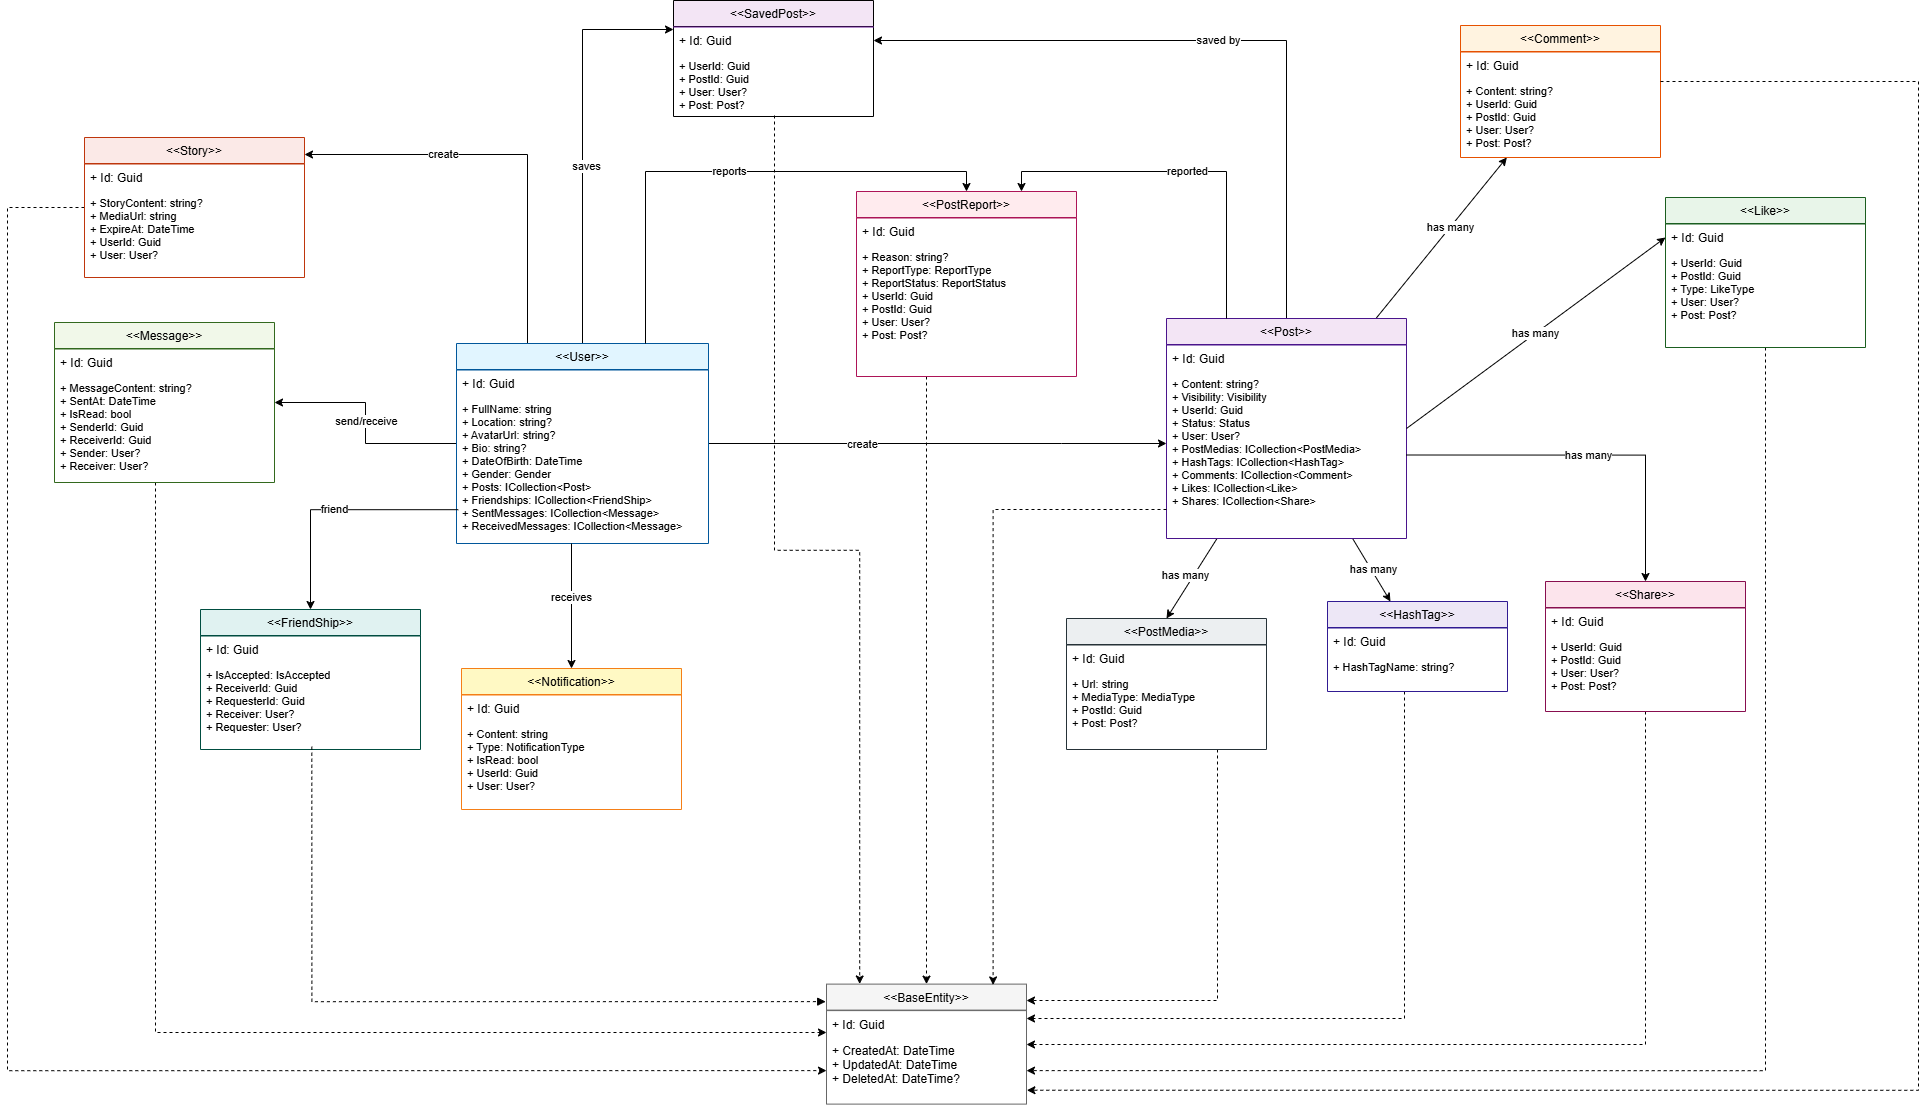
\includegraphics[width=15cm]{hinh1.drawio.png}
    \caption{Sơ đồ thực thể (ERD) của hệ thống InteractHub}
    \end{center}
    \end{figure}

    \subsection{Đặc tả API}
    Hệ thống cung cấp hơn 20 endpoints RESTful để giao tiếp với Frontend React. Các API được chuẩn hóa theo định dạng JSON và sử dụng các mã trạng thái HTTP tiêu chuẩn (200, 201, 400, 401, 500). Các nhóm API chính bao gồm:
    \begin{itemize}
        \item \textbf{Auth API}: Đăng ký, đăng nhập và cấp phát JWT Token.
        \item \textbf{Posts API}: Thực hiện các thao tác CRUD bài viết và upload hình ảnh.
        \item \textbf{Users \& Friends API}: Quản lý hồ sơ cá nhân và các yêu cầu kết bạn.
        \item \textbf{SignalR Hub}: Cung cấp các kết nối thời gian thực cho thông báo.
    \end{itemize}
    Dữ liệu truyền tải được đóng gói thông qua các lớp DTO (Data Transfer Objects) để tối ưu hóa hiệu suất và bảo mật.

    \subsection{Kiến trúc Backend}
    Phần Backend được xây dựng trên nền tảng ASP.NET Core 8.0, tuân thủ nghiêm ngặt các nguyên lý SOLID và mẫu thiết kế hiện đại:
    \begin{itemize}
        \item \textbf{Repository Pattern}: Tách biệt logic truy xuất dữ liệu khỏi logic nghiệp vụ, giúp dễ dàng bảo trì và kiểm thử.
        \item \textbf{Service Layer}: Nơi tập trung xử lý các nghiệp vụ phức tạp của hệ thống.
        \item \textbf{Dependency Injection}: Quản lý vòng đời của các đối tượng và giảm sự phụ thuộc giữa các thành phần.
        \item \textbf{Entity Framework Core}: Sử dụng kiến trúc Code-First để quản lý migration và tương tác với SQL Server.
    \end{itemize}

    % Hình kiến trúc backend được gom vào phần ảnh giao diện (xem mục "Ảnh giao diện")

    \subsection{Phân tích luồng nghiệp vụ chính (Use-case Flows)}
    Để hệ thống vận hành ổn định, nhóm xác định và hiện thực các luồng nghiệp vụ cốt lõi theo thứ tự ưu tiên từ cao xuống thấp. Mỗi luồng đều được mô tả bằng các bước xử lý ở cả frontend và backend nhằm đảm bảo tính nhất quán dữ liệu.

    \subsubsection{Luồng xác thực và khởi tạo phiên làm việc}
    \begin{enumerate}
        \item Người dùng nhập email và mật khẩu tại giao diện đăng nhập.
        \item Frontend gửi yêu cầu \texttt{POST /api/auth/login}.
        \item Backend kiểm tra thông tin người dùng qua Identity, phát hành JWT nếu hợp lệ.
        \item Frontend lưu token, gọi \texttt{/api/auth/profile} để lấy đầy đủ roles và thông tin hồ sơ.
        \item Router guard phân quyền điều hướng về trang tương ứng (User/Admin).
    \end{enumerate}

    \subsubsection{Luồng tạo bài viết có media}
    \begin{enumerate}
        \item Người dùng mở modal tạo bài viết và chọn nội dung media.
        \item Frontend upload file qua \texttt{/api/media/upload}, nhận lại URL tài nguyên.
        \item Frontend gửi dữ liệu bài viết gồm content, visibility và danh sách media URL.
        \item Backend validate dữ liệu, ghi nhận vào Post và PostMedia, trả về object chuẩn hóa.
        \item Feed được đồng bộ lại để hiển thị bài viết mới theo thời gian thực gần nhất.
    \end{enumerate}

    \subsubsection{Luồng tương tác xã hội (Like/Comment/Share)}
    \begin{itemize}
        \item Người dùng thao tác trên PostCard và nhận phản hồi tức thời (optimistic UI).
        \item API cập nhật trạng thái tương tác, đồng thời tạo Notification cho chủ bài viết nếu cần.
        \item Dữ liệu số lượng like/comment/share được cập nhật đồng bộ ở feed và trang chi tiết.
    \end{itemize}

    % Sequence diagrams moved to the unified "Ảnh giao diện" section as placeholders


%%%%%%%%%%%%%%%%%%%%%%%%%%%%%%%%%
\section{Hiện thực hóa và kết quả}

    \subsection{Frontend - Kiến trúc thành phần và giao diện đáp ứng}
    Phần Frontend được xây dựng với React 18 và TypeScript, tuân thủ nguyên tắc Component-Based Architecture:
    \begin{itemize}
        \item \textbf{Cấu trúc thành phần}: Dự án tổ chức 15+ thành phần React tái sử dụng được bao gồm:
        \begin{enumerate}
            \item Thành phần xác thực (auth): Login, Registration, Password recovery
            \item Thành phần bài viết (post): PostCard, PostForm, PostDetail, PostComments
            \item Thành phần bạn bè (friends): FriendList, FriendRequest, FriendSuggestion
            \item Thành phần thông báo (notifications): NotificationBell, NotificationPanel
            \item Thành phần khám phá (explore): UserSearch, TrendingHashtags
            \item Thành phần cài đặt (settings): ProfileSettings, PrivacySettings
            \item Thành phần tin tạm thời (story): StoryViewer, StoryUploader
            \item Thành phần gợi ý (suggestion): UserSuggestions, TrendingPosts
        \end{enumerate}
        \item \textbf{Responsive Design}: Sử dụng Tailwind CSS để đảm bảo giao diện đáp ứng hoàn hảo trên các thiết bị di động, máy tính bảng và máy tính để bàn.
        \item \textbf{React Hooks}: Sử dụng useState, useEffect, useContext, useCallback để quản lý trạng thái và hiệu ứng component.
    \end{itemize}

    \subsubsection{Cấu trúc thư mục Frontend (Folder Structure)}
    Dự án Frontend được tổ chức theo cấu trúc logic sau:
    \begin{verbatim}
    frontend/
    ├── src/
    │   ├── components/          # Các component tái sử dụng
    │   │   ├── auth/
    │   │   │   ├── Login.tsx
    │   │   │   ├── Register.tsx
    │   │   │   └── PasswordRecovery.tsx
    │   │   ├── post/
    │   │   │   ├── PostCard.tsx
    │   │   │   ├── PostForm.tsx
    │   │   │   └── PostDetail.tsx
    │   │   ├── friends/
    │   │   ├── notifications/
    │   │   ├── explore/
    │   │   ├── settings/
    │   │   ├── story/
    │   │   └── common/          # Shared components (Header, Footer, etc)
    │   ├── pages/               # Page-level components
    │   │   ├── FeedPage.tsx
    │   │   ├── ProfilePage.tsx
    │   │   ├── ExplorePage.tsx
    │   │   └── AdminPage.tsx
    │   ├── layouts/             # Layout wrappers
    │   │   ├── MainLayout.tsx
    │   │   ├── AuthLayout.tsx
    │   │   └── AdminLayout.tsx
    │   ├── services/            # API service layer
    │   │   ├── authService.ts
    │   │   ├── postService.ts
    │   │   ├── commentService.ts
    │   │   └── ...
    │   ├── contexts/            # React Context (AuthContext, etc)
    │   │   └── AuthContext.tsx
    │   ├── hooks/               # Custom React hooks
    │   │   ├── useAuth.ts
    │   │   ├── useProtectedRoute.ts
    │   │   └── useApi.ts
    │   ├── types/               # TypeScript type definitions
    │   │   ├── user.ts
    │   │   ├── post.ts
    │   │   └── api.ts
    │   ├── utils/               # Utility functions
    │   │   ├── validators.ts
    │   │   ├── formatters.ts
    │   │   └── constants.ts
    │   ├── App.tsx
    │   ├── App.css
    │   └── main.tsx
    │   └── index.css
    ├── public/
    ├── package.json
    └── tsconfig.json
    \end{verbatim}

    \subsubsection{Sơ đồ phân cấp Component (Component Hierarchy)}
    Quan hệ cha-con giữa các component chính trong ứng dụng:
    \begin{verbatim}
    App
    ├── AuthContext (Provider)
    ├── Router
    │   ├── Public Routes
    │   │   ├── LoginPage
    │   │   │   └── Login
    │   │   └── RegisterPage
    │   │       └── Register
    │   ├── Protected Routes (MainLayout)
    │   │   ├── Navbar
    │   │   │   ├── Logo
    │   │   │   ├── SearchBar
    │   │   │   └── UserMenu
    │   │   ├── Feed
    │   │   │   ├── PostForm
    │   │   │   └── PostCard (có nhiều instances)
    │   │   │       ├── PostHeader
    │   │   │       ├── PostContent
    │   │   │       ├── PostActions
    │   │   │       │   ├── LikeButton
    │   │   │       │   ├── CommentButton
    │   │   │       │   └── ShareButton
    │   │   │       └── Comments
    │   │   │           └── CommentItem
    │   │   ├── Sidebar
    │   │   │   ├── FriendList
    │   │   │   └── Suggestions
    │   │   ├── Profile
    │   │   │   ├── ProfileHeader
    │   │   │   ├── ProfileStats
    │   │   │   └── UserPosts
    │   │   ├── Explore
    │   │   │   ├── TrendingPosts
    │   │   │   ├── Hashtags
    │   │   │   └── Reels
    │   │   └── NotificationBell
    │   │       └── NotificationPanel
    │   └── Admin Routes (AdminLayout)
    │       ├── AdminDashboard
    │       ├── ReportManagement
    │       └── UserManagement
    │   └── Footer
    \end{verbatim}
    \begin{itemize}
        \item \textbf{AuthContext}: Triển khai React Context để quản lý trạng thái xác thực toàn cục, bao gồm thông tin người dùng, JWT token và trạng thái đăng nhập.
        \item \textbf{API Service Layer}: Tạo các service tách biệt cho từng miền nghiệp vụ:
        \begin{enumerate}
            \item authService.ts - Xử lý đăng ký, đăng nhập, làm mới token
            \item postService.ts - CRUD operations cho bài viết
            \item commentService.ts - Quản lý bình luận
            \item likeService.ts - Quản lý lượt thích
            \item friendService.ts - Quản lý yêu cầu kết bạn
            \item notificationService.ts - Lấy thông báo
            \item storyService.ts - Quản lý tin tạm thời
            \item shareService.ts - Chia sẻ bài viết
            \item userService.ts - Quản lý hồ sơ người dùng
        \end{enumerate}
        \item \textbf{API Interceptor}: Tự động đính kèm JWT token vào headers của tất cả requests.
        \item \textbf{Error Handling}: Xử lý lỗi API toàn cục với thông báo lỗi rõ ràng cho người dùng.
    \end{itemize}

    \subsection{Frontend - Forms với xác thực}
    \begin{itemize}
        \item \textbf{React Hook Form}: Triển khai các form bao gồm:
        \begin{enumerate}
            \item Form đăng ký: Xác thực email, mật khẩu mạnh, xác nhận mật khẩu
            \item Form đăng nhập: Email/mật khẩu với xử lý lỗi
            \item Form tạo bài viết: Hỗ trợ upload hình ảnh với preview
            \item Form cập nhật hồ sơ: Thay đổi avatar, bio, thông tin cá nhân
        \end{enumerate}
        \item \textbf{Validation}: Kiểm tra phía client bao gồm:
        \begin{enumerate}
            \item Định dạng email (regex)
            \item Độ mạnh mật khẩu (ký tự hoa, chữ số, ký tự đặc biệt, ít nhất 8 ký tự)
            \item Kiểm tra trùng lặp email khi đăng ký
            \item Giới hạn kích thước file hình ảnh
        \end{enumerate}
        \item \textbf{User Experience}: Loading states, success/error messages, form validation feedback real-time.
    \end{itemize}

    % Form screenshots moved to the unified "Ảnh giao diện" section

    \subsection{Frontend - Routing và Dynamic Features}
    \begin{itemize}
        \item \textbf{React Router v6}: Cấu hình route nested bao gồm:
        \begin{enumerate}
            \item Public routes: /login, /register, /home (không yêu cầu xác thực)
            \item Protected routes: /feed, /profile, /friends, /messages (yêu cầu xác thực)
            \item Admin routes: /admin/reports, /admin/users
        \end{enumerate}
        \item \textbf{Route Guards}: Custom hook \texttt{useProtectedRoute} để chuyển hướng người dùng chưa xác thực tới trang login.
        \item \textbf{Search với Debouncing}: Tìm kiếm người dùng, hashtags với debounce delay 300ms để giảm số lượng API calls.
        \item \textbf{Pagination/Infinite Scroll}: Tải bài viết động với infinite scroll thay vì phân trang truyền thống.
        \item \textbf{Lazy Loading}: Lazy-loaded routes bằng React.lazy() giảm kích thước bundle ban đầu.
        \item \textbf{Real-time Notifications}: Tích hợp SignalR client để nhận thông báo ngay lập tức từ server.
    \end{itemize}

    

    \subsection{Chức năng xác thực Backend (Authentication \& Authorization)}
    Hệ thống sử dụng \textbf{ASP.NET Core Identity} kết hợp với \textbf{JSON Web Token (JWT)} để quản lý người dùng và bảo mật API:
    \begin{itemize}
        \item \textbf{Đăng ký và Đăng nhập}: 
        \begin{enumerate}
            \item Endpoint: \texttt{POST /api/auth/register} - Tạo tài khoản mới với email/password
            \item Endpoint: \texttt{POST /api/auth/login} - Xác thực và trả về JWT token
            \item Password hashing tự động bằng Identity
        \end{enumerate}
        \item \textbf{JWT Token Generation}: 
        \begin{enumerate}
            \item Token chứa claims: UserId, Email, Roles
            \item Expiration: 24 giờ (có thể cấu hình)
            \item Lưu trữ ở Client-side trong localStorage/sessionStorage
        \end{enumerate}
        \item \textbf{Authorization}: Sử dụng \texttt{[Authorize]} attribute trên controllers để bảo vệ endpoints.
        \item \textbf{Role-based Access}: Admin role có quyền xóa bài viết, quản lý báo cáo; User role có quyền tạo bài viết cá nhân.
    \end{itemize}

    \subsection{Database Design và Entity Framework Core}
    Hệ thống được thiết kế với \textbf{9 entities chính}:
    \begin{enumerate}
        \item \textbf{User} (AspNetUsers): Người dùng, tích hợp ASP.NET Core Identity
        \item \textbf{Post}: Bài viết với Content, CreatedAt, UserId (Foreign Key)
        \item \textbf{Comment}: Bình luận trên bài viết
        \item \textbf{Like}: Lượt thích bài viết
        \item \textbf{Friendship}: Mối quan hệ bạn bè với status (Pending, Accepted, Blocked)
        \item \textbf{Story}: Tin tạm thời với expiration (24 giờ)
        \item \textbf{Notification}: Thông báo với type (Like, Comment, FriendRequest)
        \item \textbf{Hashtag}: Theo dõi hashtag xu hướng
        \item \textbf{PostReport}: Báo cáo nội dung vi phạm
    \end{enumerate}

    % Hình (hinh7.png) được loại bỏ khỏi nội dung chính; giữ mô tả để chèn sau ở phần "Ảnh giao diện".

    \subsubsection{Cấu trúc thư mục Backend (Folder Structure)}
    Dự án Backend được tổ chức theo kiến trúc phân lớp sau:
    \begin{verbatim}
    backend/
    ├── InteractHub.Api/
    │   ├── Controllers/         # API Controllers (11 controllers)
    │   │   ├── AuthController.cs
    │   │   ├── PostController.cs
    │   │   ├── CommentController.cs
    │   │   ├── LikeController.cs
    │   │   ├── FriendshipController.cs
    │   │   ├── NotificationController.cs
    │   │   ├── StoryController.cs
    │   │   ├── ShareController.cs
    │   │   ├── UserController.cs
    │   │   ├── MessageController.cs
    │   │   └── MediaController.cs
    │   ├── Services/            # Business Logic (12 services)
    │   │   ├── Interfaces/
    │   │   │   ├── IAuthService.cs
    │   │   │   ├── IPostService.cs
    │   │   │   ├── ICommentService.cs
    │   │   │   ├── ILikeService.cs
    │   │   │   ├── IFriendshipService.cs
    │   │   │   ├── INotificationService.cs
    │   │   │   ├── IStoryService.cs
    │   │   │   ├── IShareService.cs
    │   │   │   ├── IUserService.cs
    │   │   │   ├── IMessageService.cs
    │   │   │   ├── IFileUploadService.cs
    │   │   │   └── ISavedPostService.cs
    │   │   └── Implementations/
    │   │       ├── AuthService.cs
    │   │       ├── PostService.cs
    │   │       └── ... (mỗi service implement tương ứng)
    │   ├── Repositories/        # Data Access Layer
    │   │   ├── Interfaces/
    │   │   │   ├── IPostRepository.cs
    │   │   │   ├── ICommentRepository.cs
    │   │   │   └── ...
    │   │   └── Implementations/
    │   │       ├── PostRepository.cs
    │   │       └── ...
    │   ├── Data/                # Database Context
    │   │   ├── ApplicationDbContext.cs
    │   │   ├── DataContextDapper.cs
    │   │   └── DataSeeder.cs
    │   ├── Models/              # Entity Models (9 entities)
    │   │   ├── User.cs
    │   │   ├── Post.cs
    │   │   ├── Comment.cs
    │   │   ├── Like.cs
    │   │   ├── Friendship.cs
    │   │   ├── Story.cs
    │   │   ├── Notification.cs
    │   │   ├── Hashtag.cs
    │   │   └── PostReport.cs
    │   ├── DTOs/                # Data Transfer Objects
    │   │   ├── Auth/
    │   │   ├── Post/
    │   │   ├── Comment/
    │   │   └── ...
    │   ├── Migrations/          # Entity Framework Migrations
    │   ├── Program.cs           # Cấu hình DI, CORS, etc
    │   ├── appsettings.json
    │   ├── appsettings.Development.json
    │   ├── Dockerfile
    │   └── InteractHub.Api.csproj
    │
    └── InteractHub.Tests/       # Unit Testing Project
        ├── AuthControllerTests.cs
        ├── AuthServiceTests.cs
        ├── PostServiceTests.cs
        ├── CommentServiceTests.cs
        ├── LikeServiceTests.cs
        ├── FriendshipServiceTests.cs
        ├── ShareServiceTests.cs
        ├── StoryServiceTests.cs
        ├── MessageServiceTests.cs
        ├── NotificationServiceTests.cs
        ├── NotificationsControllerTests.cs
        ├── UserServiceTests.cs
        ├── FileUploadServiceTests.cs
        └── InteractHub.Tests.csproj
    \end{verbatim}
    \begin{itemize}
        \item \textbf{AuthController} (2 endpoints): Register, Login
        \item \textbf{PostController} (6 endpoints): GetAll, GetById, Create, Update, Delete, GetUserPosts
        \item \textbf{CommentController} (5 endpoints): Create, GetByPost, Update, Delete, GetAll
        \item \textbf{LikeController} (3 endpoints): AddLike, RemoveLike, GetLikeCount
        \item \textbf{FriendshipController} (5 endpoints): SendRequest, AcceptRequest, DeclineRequest, GetFriends, GetRequests
        \item \textbf{NotificationController} (3 endpoints): GetNotifications, MarkAsRead, GetUnreadCount
        \item \textbf{StoryController} (4 endpoints): CreateStory, GetStories, ViewStory, DeleteStory
        \item \textbf{ShareController} (2 endpoints): SharePost, GetShares
        \item \textbf{UserController} (4 endpoints): GetProfile, UpdateProfile, SearchUsers, GetUserStats
        \item \textbf{MessageController} (2 endpoints): SendMessage, GetMessages
        \item \textbf{MediaController} (2 endpoints): UploadImage, DeleteImage
    \end{itemize}
    \subsection{Cấu hình CORS và Dependency Injection}
    Cấu hình CORS trong \texttt{Program.cs} cho phép Frontend React giao tiếp an toàn với Backend API, đảm bảo tính bảo mật và khả năng mở rộng khi triển khai trên các môi trường khác nhau:
    \begin{lstlisting}[caption={Cấu hình CORS và Dependency Injection trong Program.cs}]
// Configure CORS
var MyAllowedOrigins = "_myAllowedOrigins";

builder.Services.AddCors(options =>
{
    options.AddPolicy(name: MyAllowedOrigins, policy =>
    {
        policy
            .WithOrigins(
                "http://localhost:3000",
                "http://localhost:5173",
                "https://interacthub-frontend.azurewebsites.net")
            .AllowAnyHeader()
            .AllowAnyMethod()
            .AllowCredentials();
    });
});

// Registering Business Logic Services (Dependency Injection)
builder.Services.AddScoped<IAuthService, AuthService>();
builder.Services.AddScoped<IPostService, PostService>();
builder.Services.AddScoped<ICommentService, CommentService>();
builder.Services.AddScoped<ILikeService, LikeService>();
builder.Services.AddScoped<IFriendshipService, FriendshipService>();
builder.Services.AddScoped<INotificationService, NotificationService>();
builder.Services.AddScoped<IStoryService, StoryService>();
builder.Services.AddScoped<IShareService, ShareService>();
builder.Services.AddScoped<IUserService, UserService>();
builder.Services.AddScoped<IMessageService, MessageService>();
builder.Services.AddScoped<IFileUploadService, FileUploadService>();
builder.Services.AddScoped<ISavedPostService, SavedPostService>();

// Add generic repository
builder.Services.AddScoped(typeof(IRepository<>), typeof(Repository<>));

var app = builder.Build();
app.UseCors(MyAllowedOrigins);
app.MapControllers();
app.Run();
    \end{lstlisting}

    Cấu hình này đảm bảo:
    \begin{itemize}
        \item \textbf{CORS Policy}: Cho phép các request từ Frontend (localhost:3000, localhost:5173, Azure domain)
        \item \textbf{Credentials}: Hỗ trợ gửi JWT token trong Cookie/Header
        \item \textbf{Dependency Injection}: Tất cả services được đăng ký với Scoped lifetime cho tính consistency trong mỗi HTTP request
        \item \textbf{Generic Repository}: Hỗ trợ các entity models thông qua generic repository pattern
    \end{itemize}

    \subsection{Business Logic và Services Layer}
    Triển khai \textbf{12 service interfaces} với implementation pattern:
    \begin{itemize}
        \item \textbf{Service Interfaces}: IAuthService, IPostService, ICommentService, ILikeService, IFriendshipService, INotificationService, IStoryService, IShareService, IUserService, IMessageService, IFileUploadService, ISavedPostService
        \item \textbf{Dependency Injection}: Tất cả services được đăng ký trong Program.cs với Scoped lifetime.
        \item \textbf{SOLID Principles}: 
        \begin{enumerate}
            \item \textit{Single Responsibility}: Mỗi service chỉ quản lý một miền nghiệp vụ
            \item \textit{Open/Closed}: Dễ mở rộng bằng cách tạo service mới mà không sửa code hiện tại
            \item \textit{Liskov Substitution}: Services implement từ interfaces chung
            \item \textit{Interface Segregation}: Interfaces tập trung vào chức năng cụ thể
            \item \textit{Dependency Inversion}: Phụ thuộc vào interfaces, không phụ thuộc vào implementations
        \end{enumerate}
    \end{itemize}

    \subsection{Lưu trữ Cloud (Azure Blob Storage)}
    \begin{itemize}
        \item \textbf{File Upload Service}: Xử lý upload hình ảnh từ React lên Azure Blob Storage.
        \item \textbf{Blob URL}: Trả về public URL của blob để hiển thị hình ảnh trên frontend.
        \item \textbf{File Validation}: Kiểm tra định dạng (.jpg, .png, .gif) và kích thước ($\leq$ 5MB).
    \end{itemize}

    \subsection{Kết quả đạt được}
    Sau thời gian triển khai và phát triển, ứng dụng InteractHub đã đạt được các kết quả cụ thể sau:
    \begin{itemize}
        \item \textbf{Frontend}: 
        \begin{enumerate}
            \item 15+ components React được xây dựng với TypeScript strict mode
            \item Giao diện responsive hoàn hảo trên desktop, tablet, mobile
            \item AuthContext quản lý trạng thái xác thực toàn cục
            \item 10 API services tích hợp tất cả endpoints backend
            \item Form validation toàn diện với React Hook Form
            \item Dynamic routing với protected routes
        \end{enumerate}
        \item \textbf{Backend}: 
        \begin{enumerate}
            \item 11 API Controllers với 20+ endpoints
            \item 12 Service Interfaces implementation
            \item JWT Authentication và Authorization hoàn chỉnh
            \item 9 Database entities được định nghĩa và migrate
            \item Swagger/OpenAPI documentation tự động
            \item CORS configuration cho React frontend
        \end{enumerate}
        \item \textbf{Code Quality}: 
        \begin{enumerate}
            \item Repository pattern cho data access
            \item Service layer tách biệt business logic
            \item DTO cho tất cả request/response
            \item Proper error handling và validation
        \end{enumerate}
    \end{itemize}

    \subsection{Minh chứng kết quả giao diện và chức năng}
    Mục này trình bày bộ ảnh giao diện thực tế từ ứng dụng InteractHub, thể hiện các chức năng chính theo nhóm tính năng.

    \subsubsection{Nhóm xác thực và hồ sơ người dùng}
    \begin{figure}[H]
    \begin{center}
    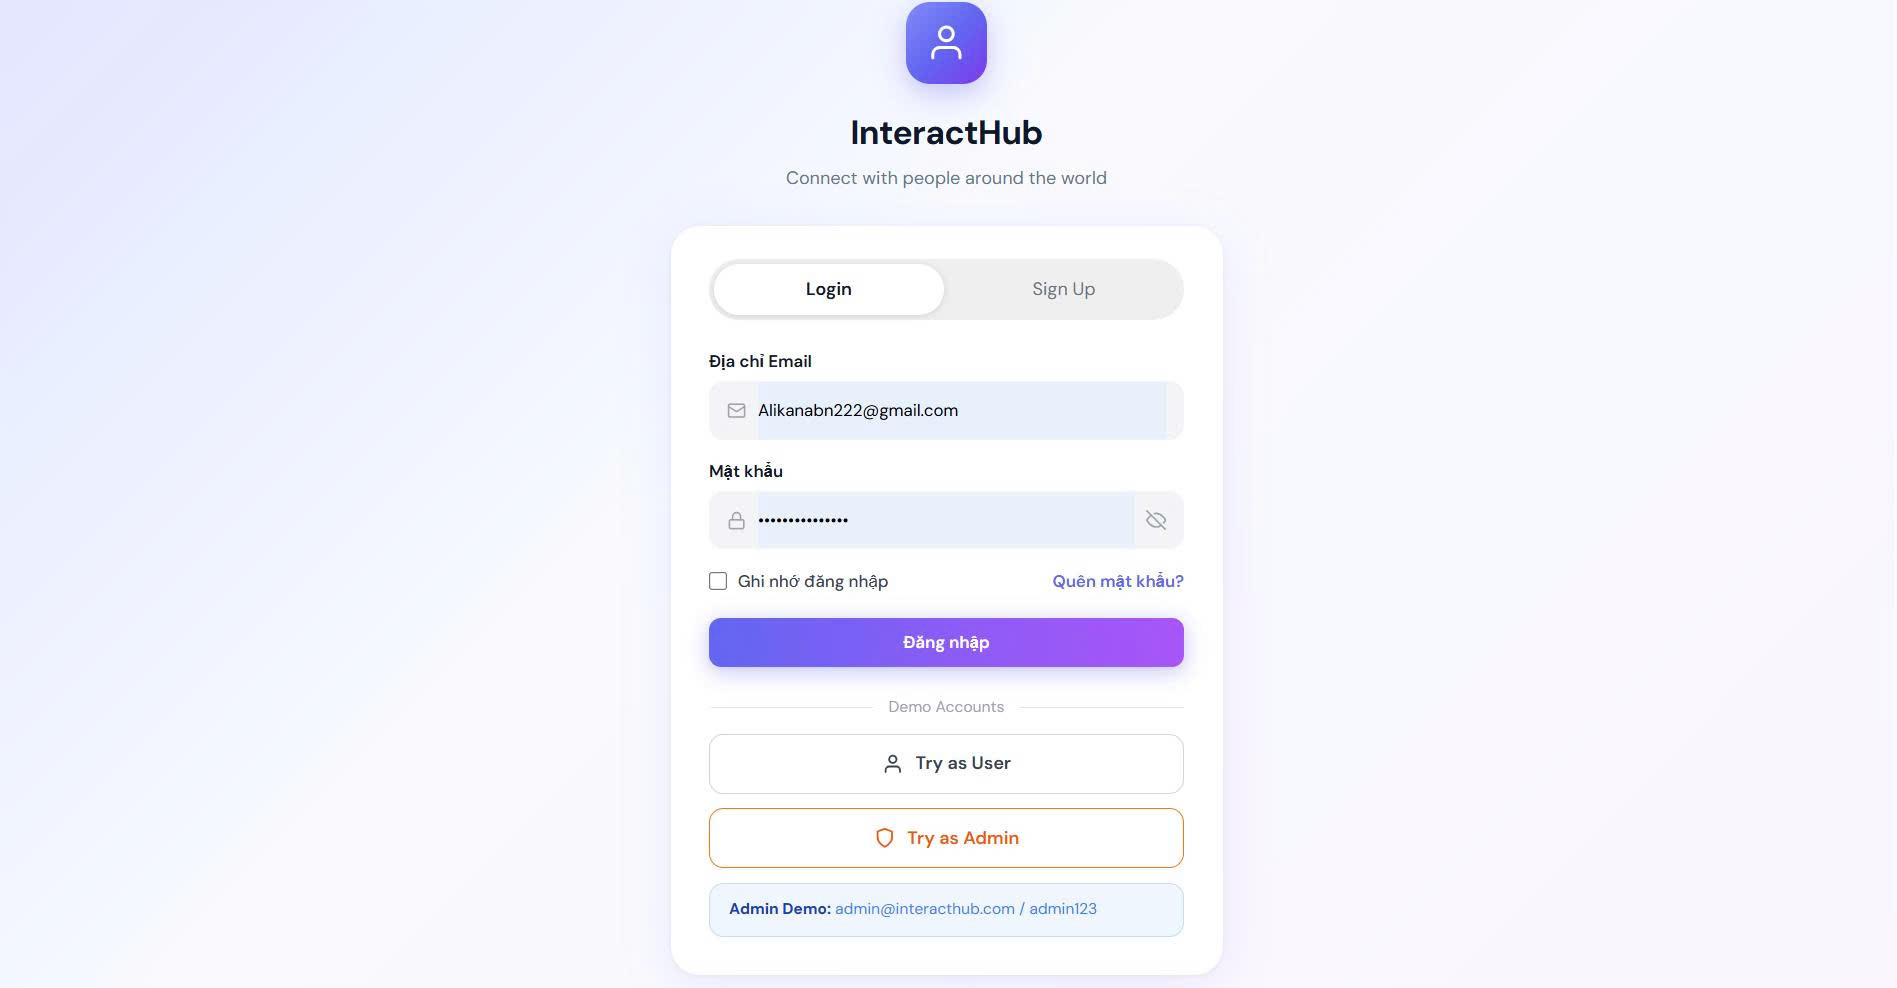
\includegraphics[width=14cm]{Trangdangnhap.png}
    \caption{Trang đăng nhập hệ thống}
    \end{center}
    \end{figure}

    \begin{figure}[H]
    \begin{center}
    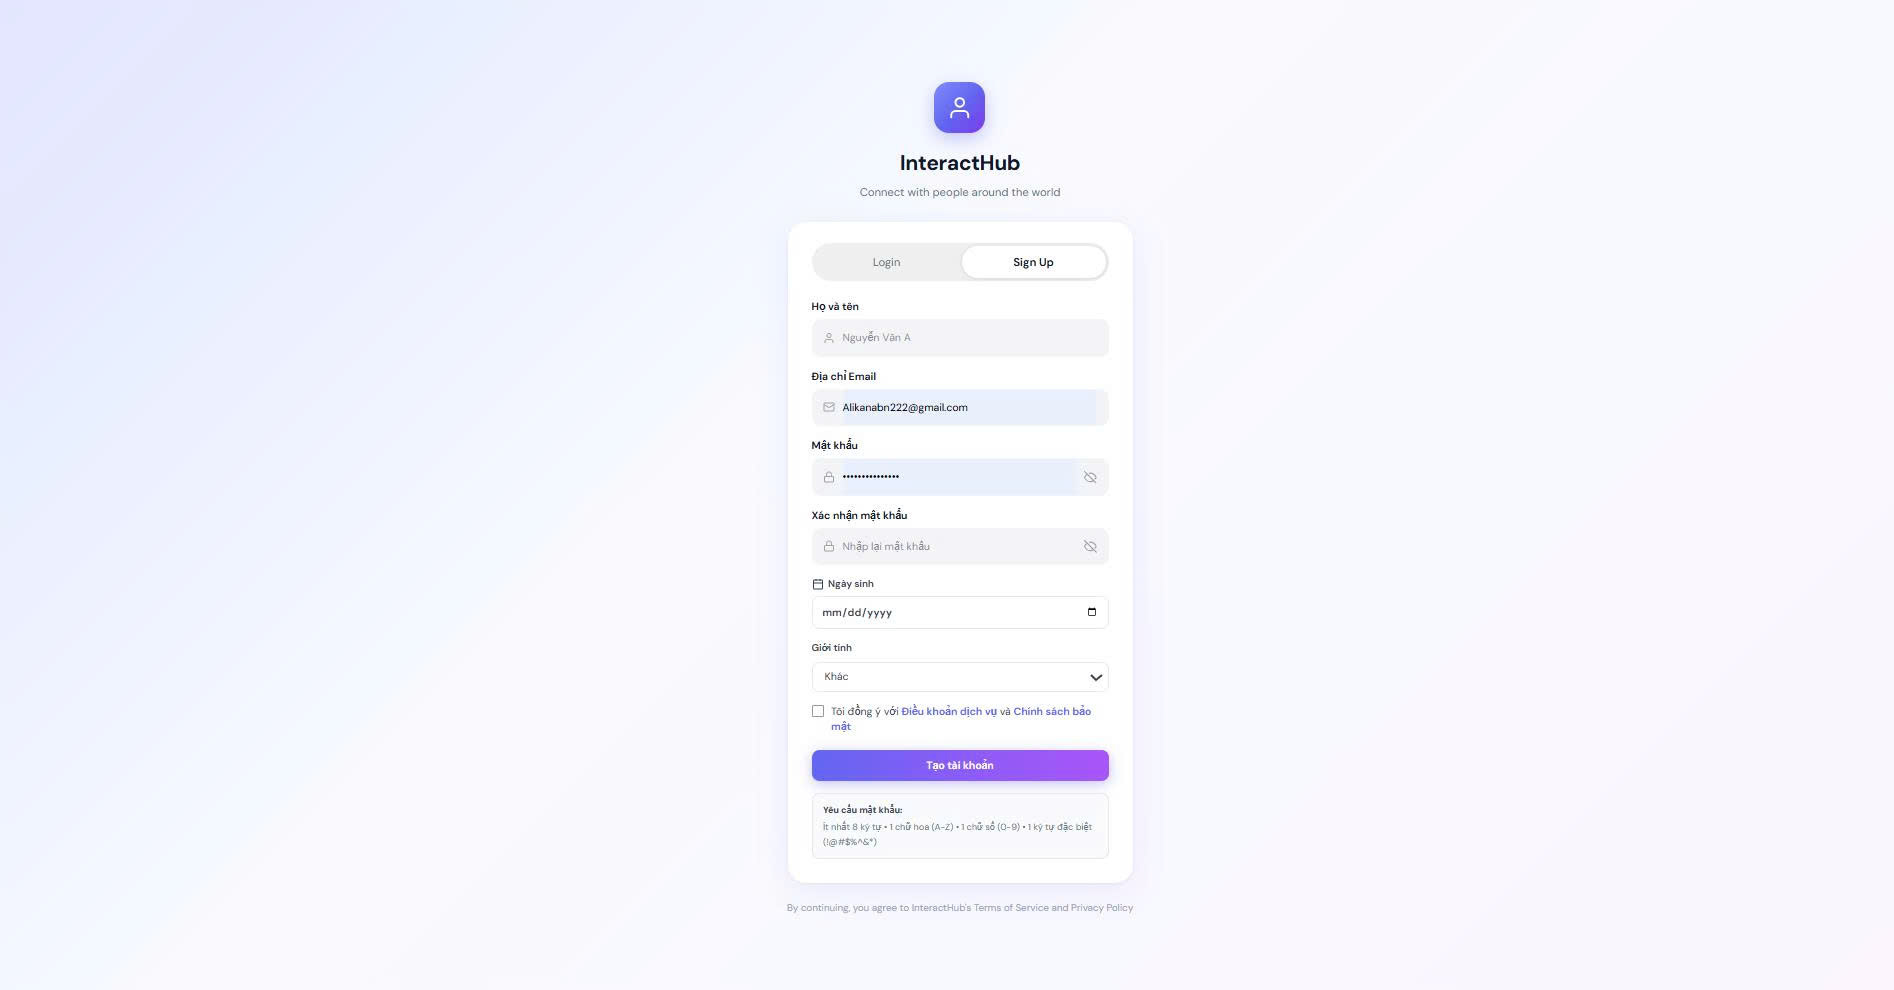
\includegraphics[width=14cm]{GiaoDienDangKiTaiKhoan.jpg}
    \caption{Giao diện đăng ký tài khoản người dùng}
    \end{center}
    \end{figure}

    \begin{figure}[H]
    \begin{center}
    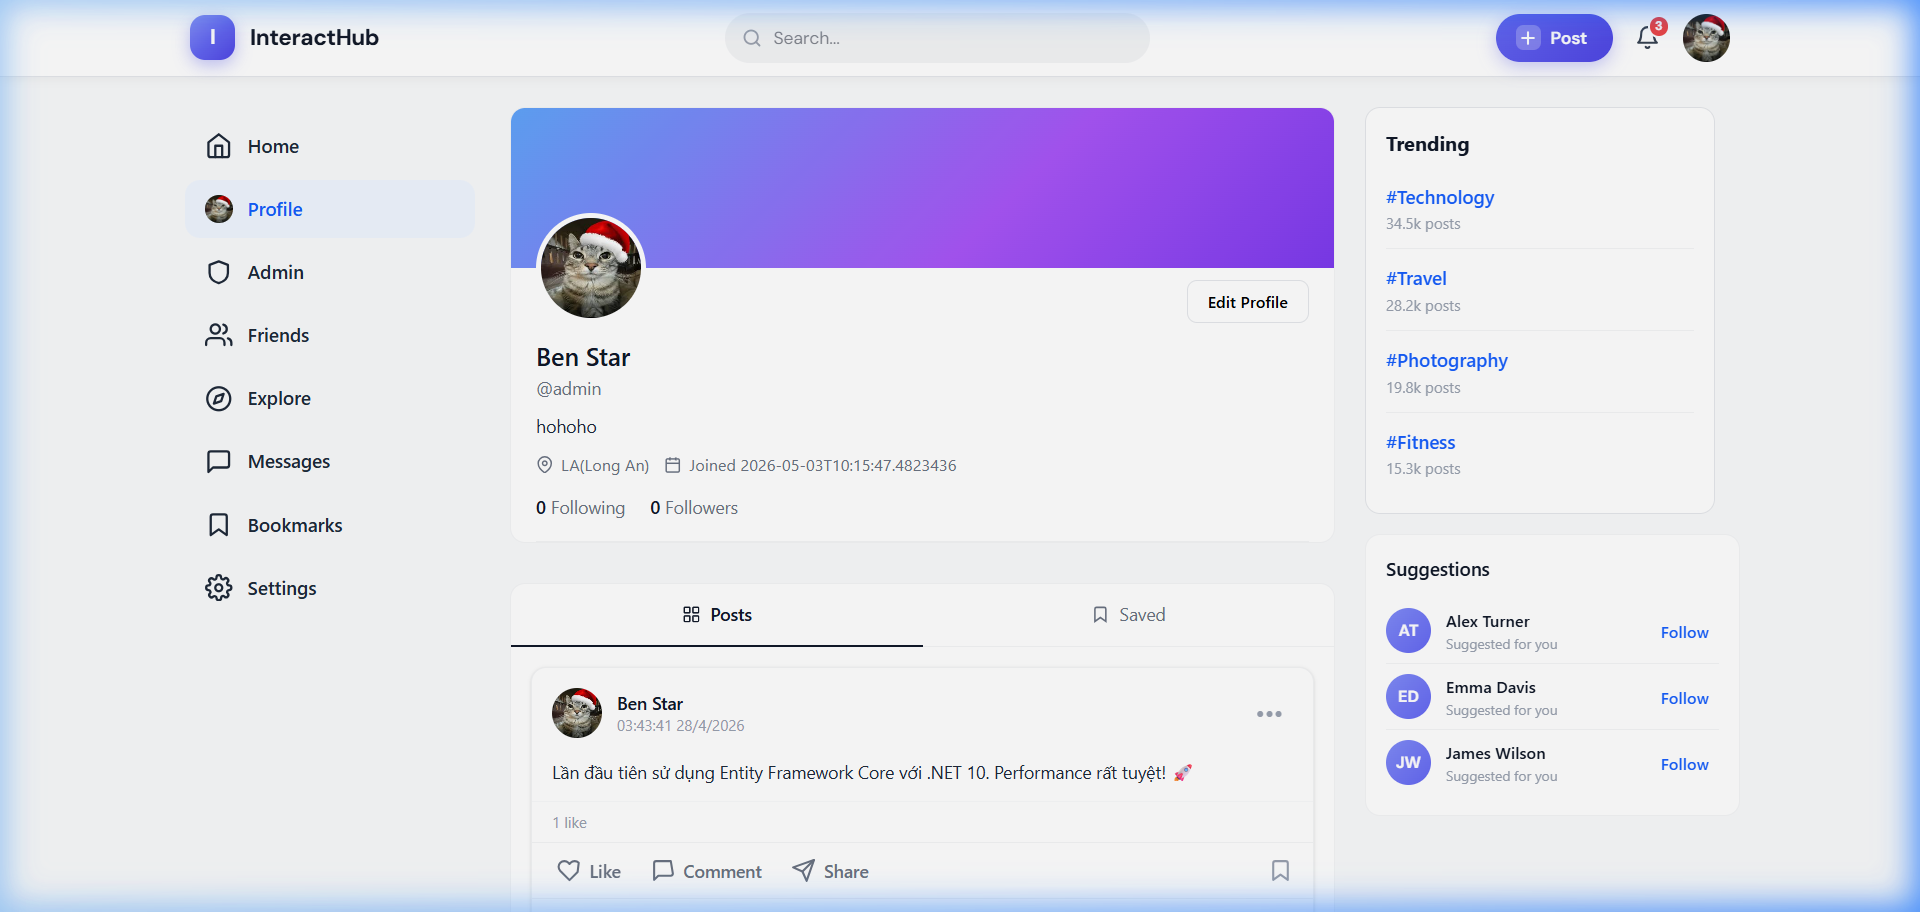
\includegraphics[width=14cm]{GiaoDienProfile.png}
    \caption{Trang hồ sơ người dùng (Profile)}
    \end{center}
    \end{figure}

    \begin{figure}[H]
    \begin{center}
    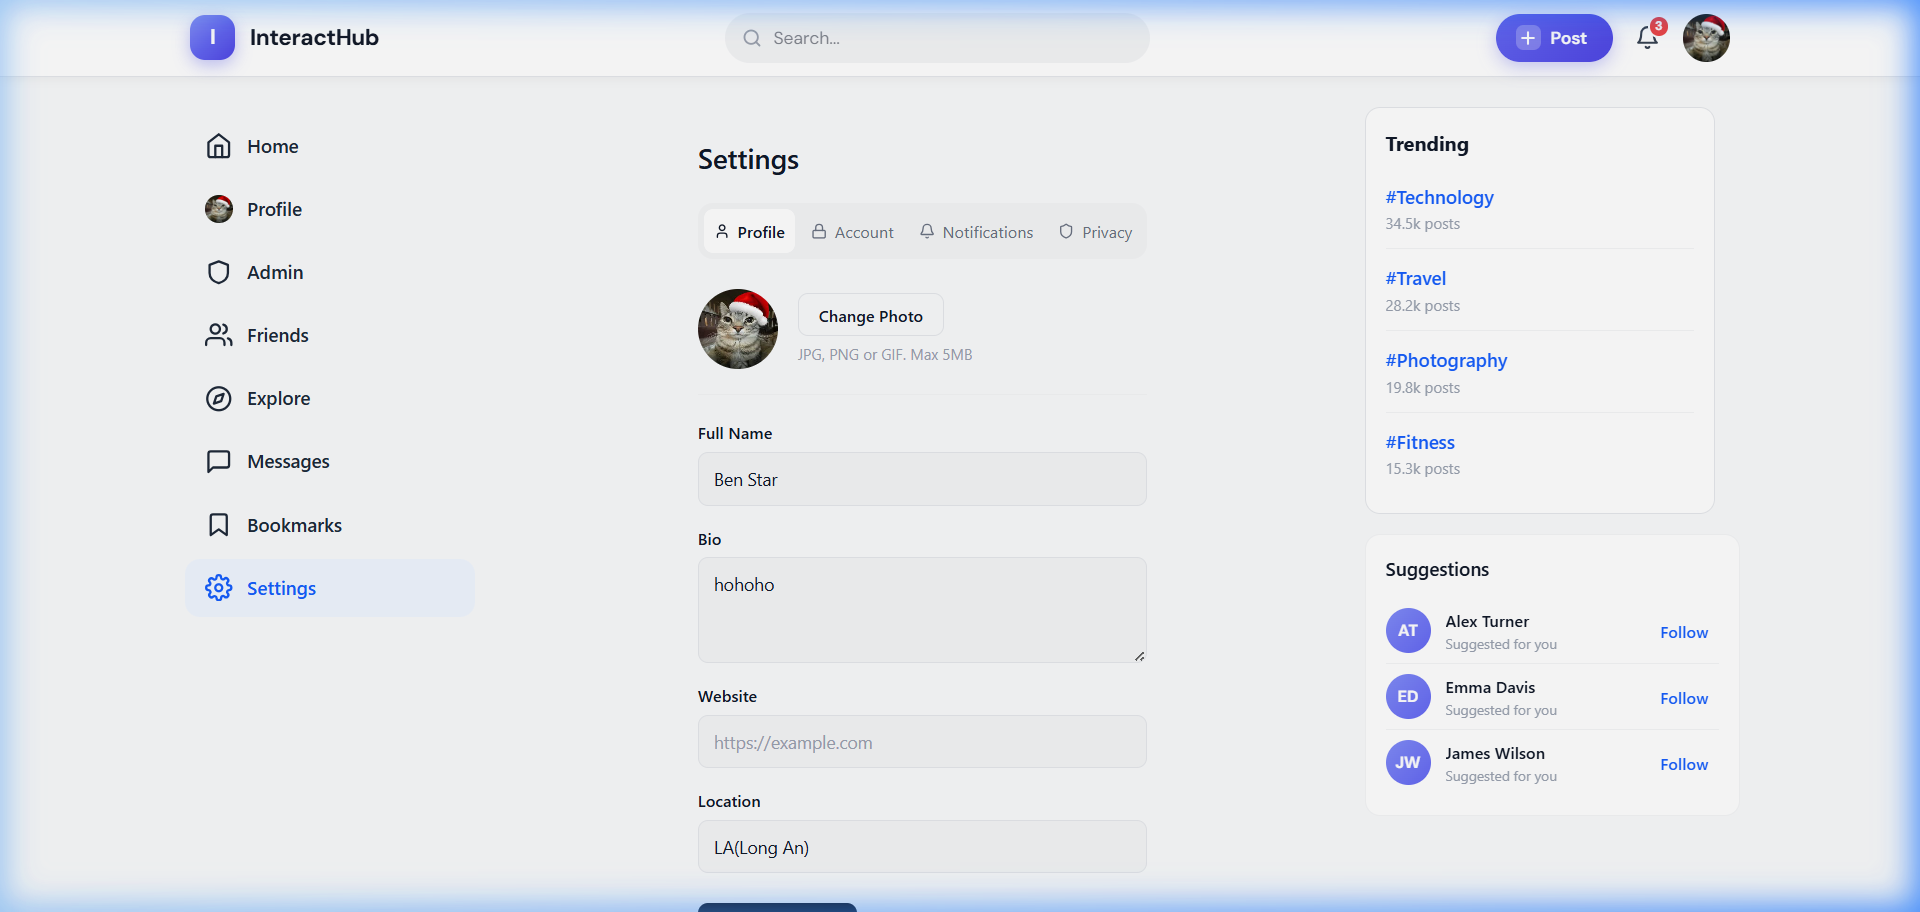
\includegraphics[width=14cm]{GiaoDienCaiDat_ProfileNguoiDung.png}
    \caption{Cài đặt hồ sơ (Settings - Profile)}
    \end{center}
    \end{figure}

    \begin{figure}[H]
    \begin{center}
    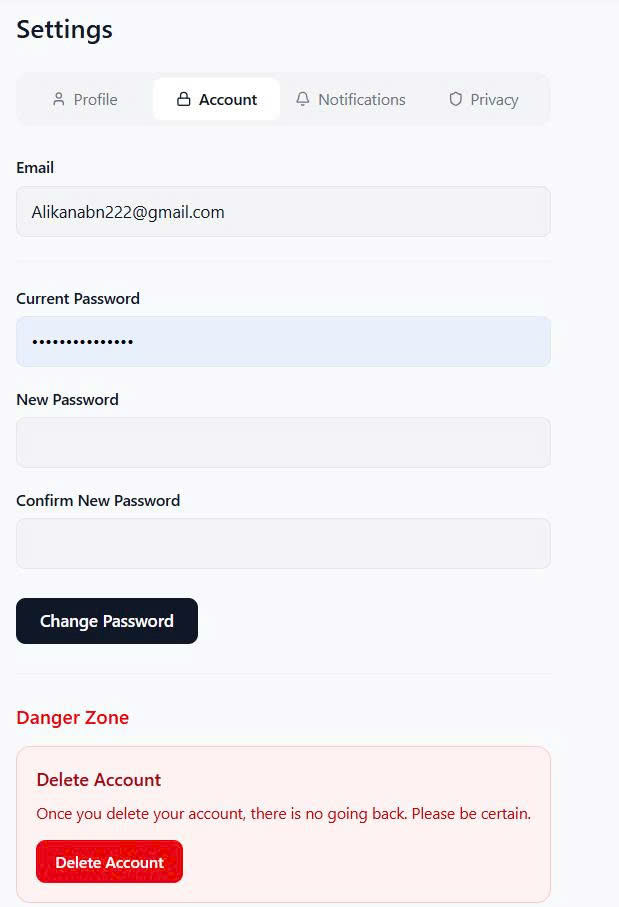
\includegraphics[width=14cm]{GiaoDienCaiDat_Account.jpg}
    \caption{Cài đặt tài khoản (Settings - Account)}
    \end{center}
    \end{figure}

    \begin{figure}[H]
    \begin{center}
    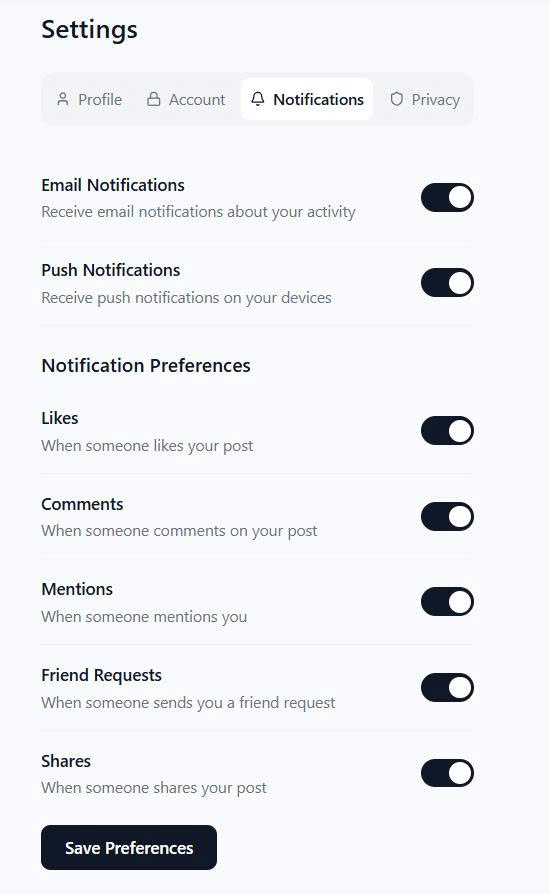
\includegraphics[width=14cm]{GiaoDienCaiDat_ThongBao.jpg}
    \caption{Cài đặt thông báo (Settings - Notifications)}
    \end{center}
    \end{figure}

    \begin{figure}[H]
    \begin{center}
    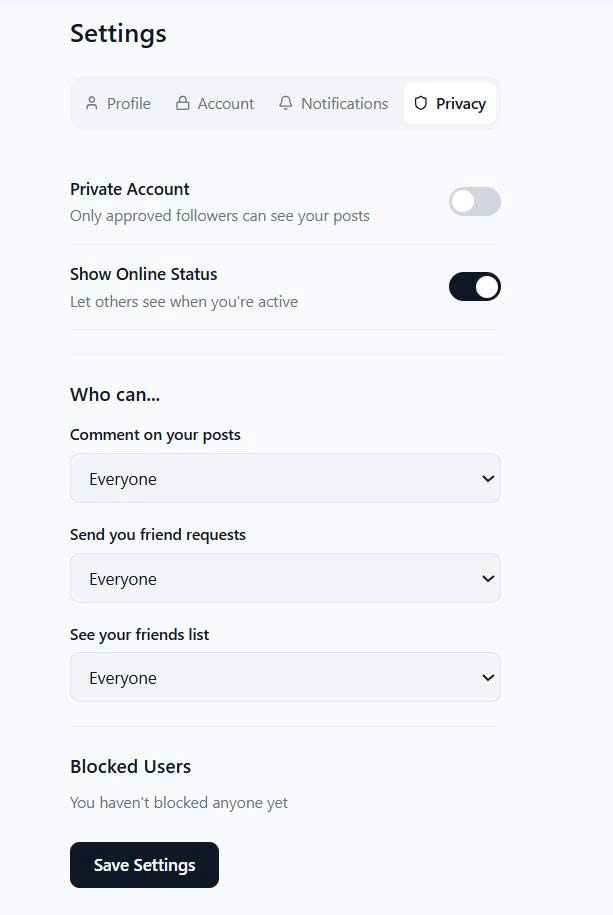
\includegraphics[width=14cm]{GiaoDienCaiDat_Privacy.jpg}
    \caption{Cài đặt quyền riêng tư (Settings - Privacy)}
    \end{center}
    \end{figure}

    \subsubsection{Nhóm feed, bài viết và story}
    \begin{figure}[H]
    \begin{center}
    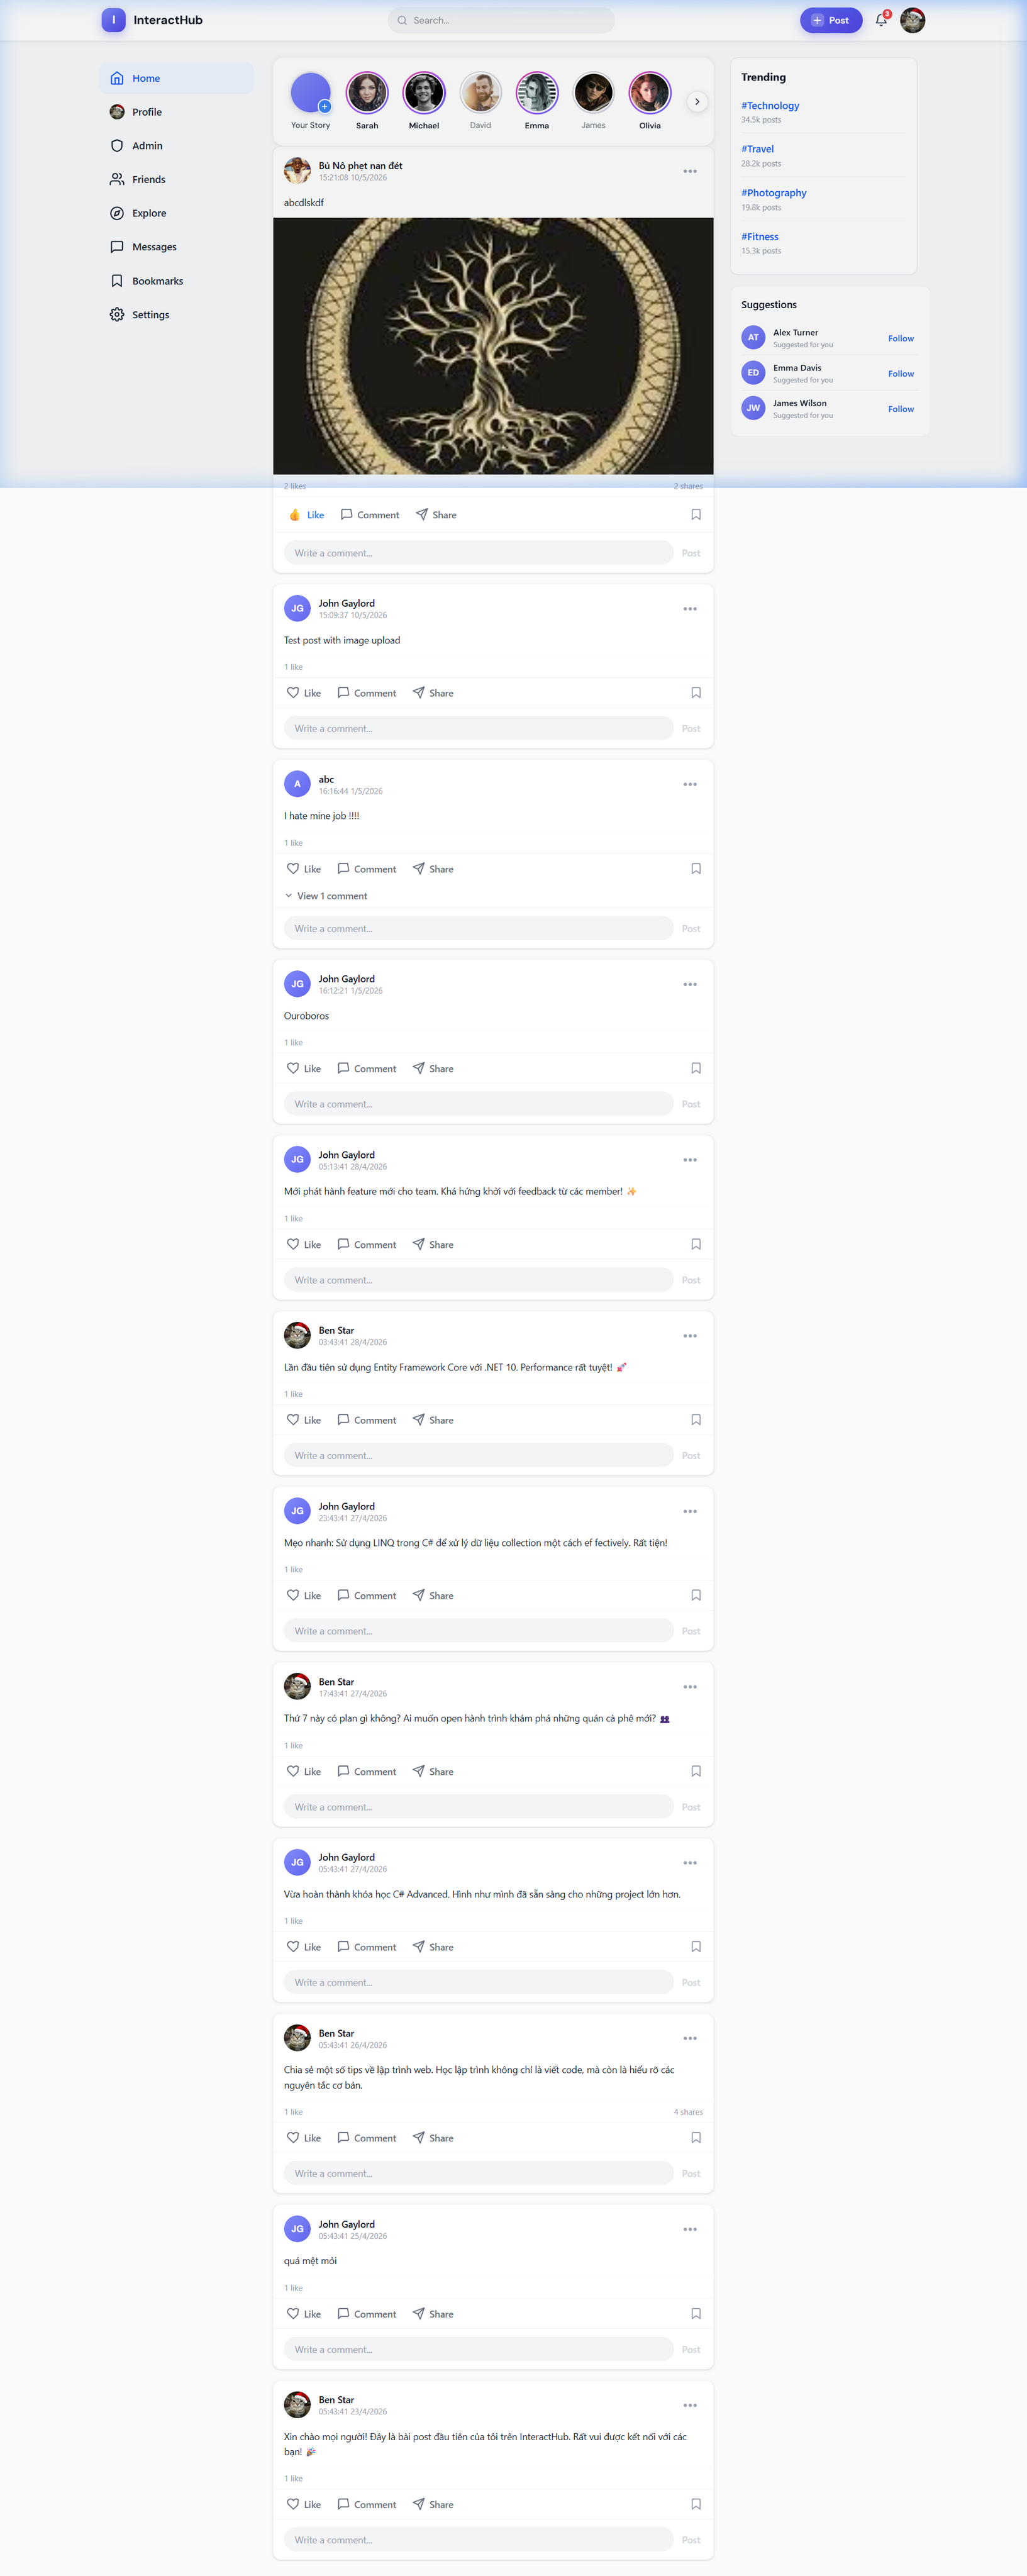
\includegraphics[width=14cm]{GiaoDienTongQuanInteractHub.png}
    \caption{Trang chủ Feed - tổng quan hệ thống sau khi đăng nhập}
    \end{center}
    \end{figure}

    \begin{figure}[H]
    \begin{center}
    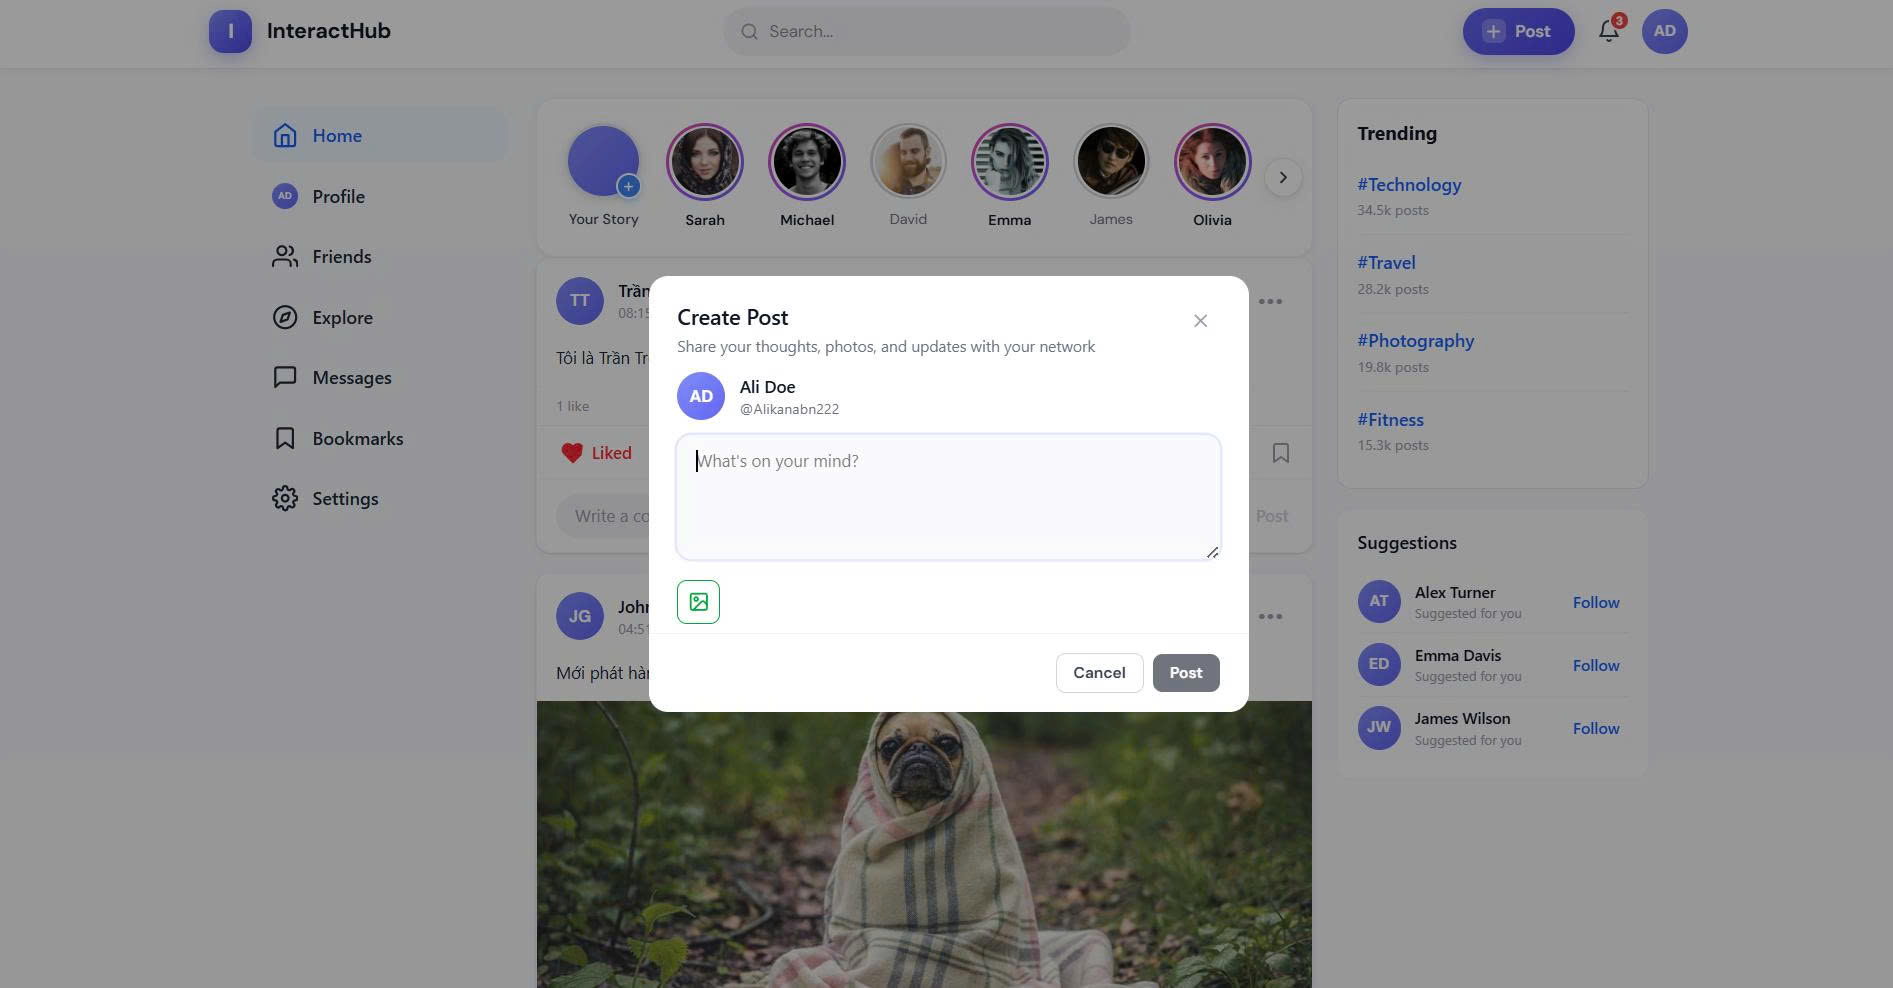
\includegraphics[width=14cm]{TaoBaiViet.jpg}
    \caption{Tạo bài viết mới (Create Post Modal)}
    \end{center}
    \end{figure}

    \begin{figure}[H]
    \begin{center}
    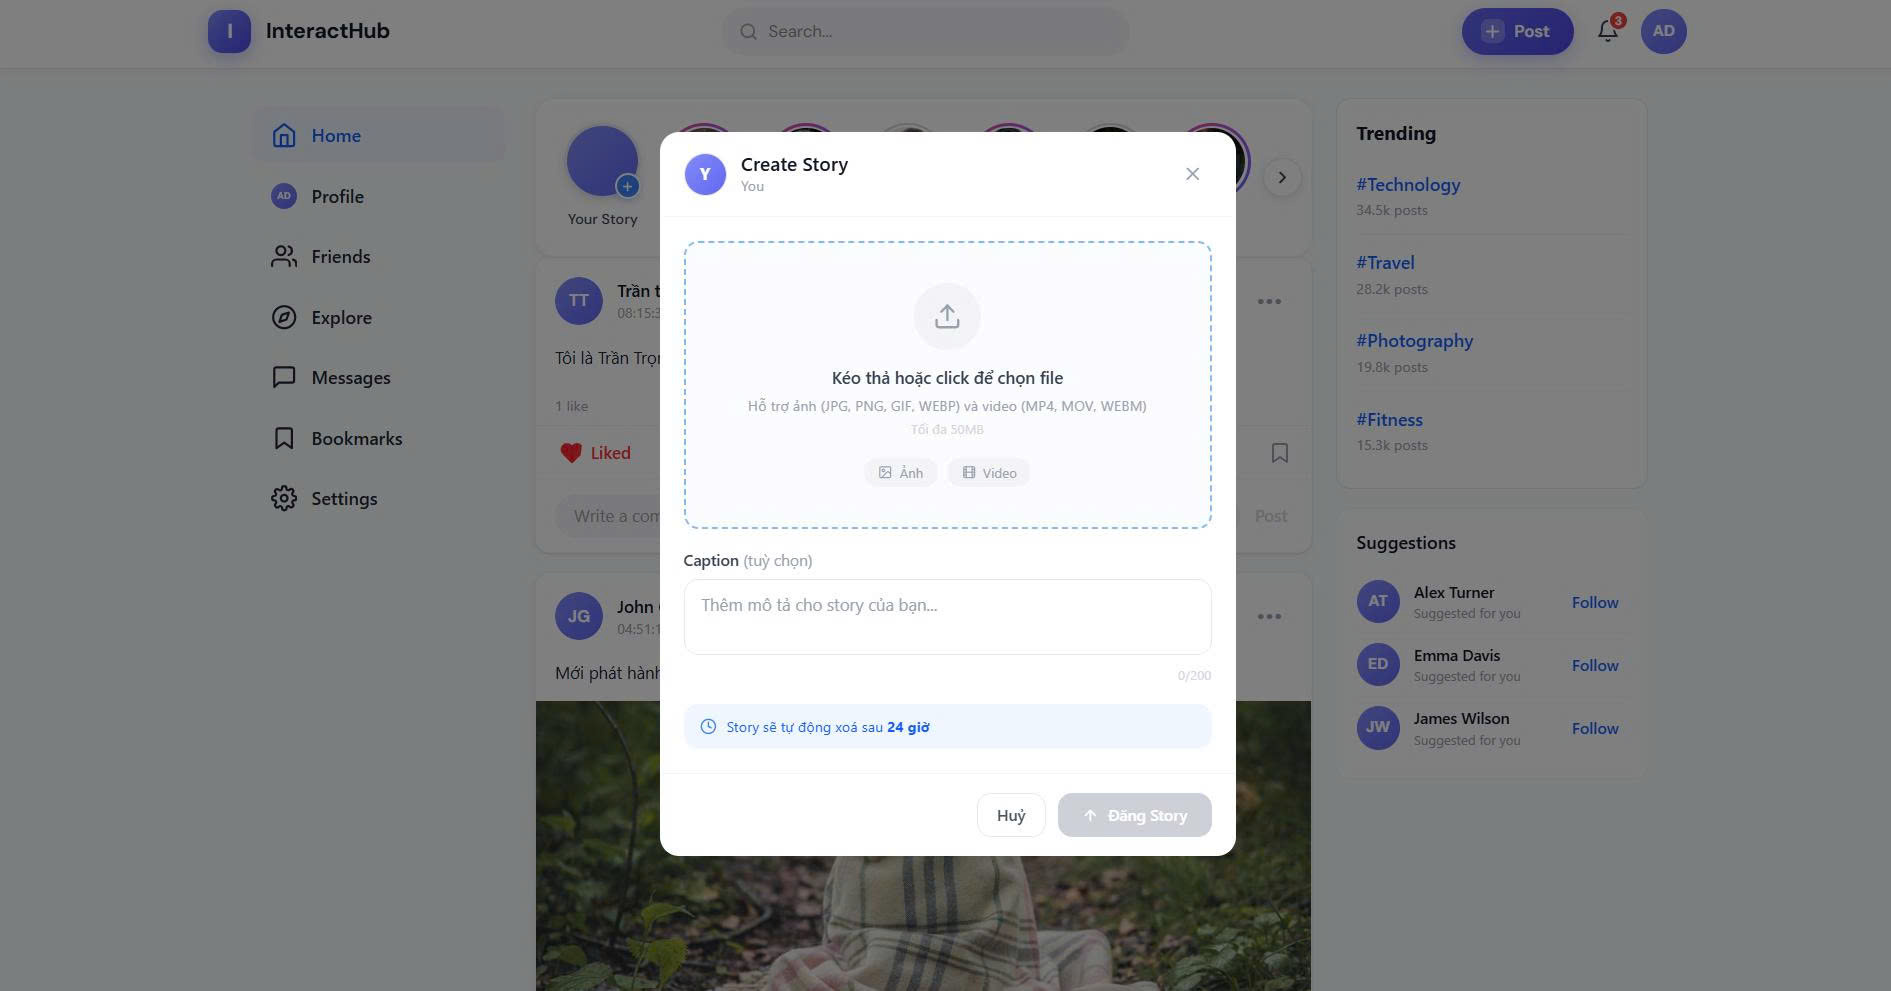
\includegraphics[width=14cm]{TaoStory.jpg}
    \caption{Tạo story mới (Create Story Modal)}
    \end{center}
    \end{figure}

    \begin{figure}[H]
    \begin{center}
    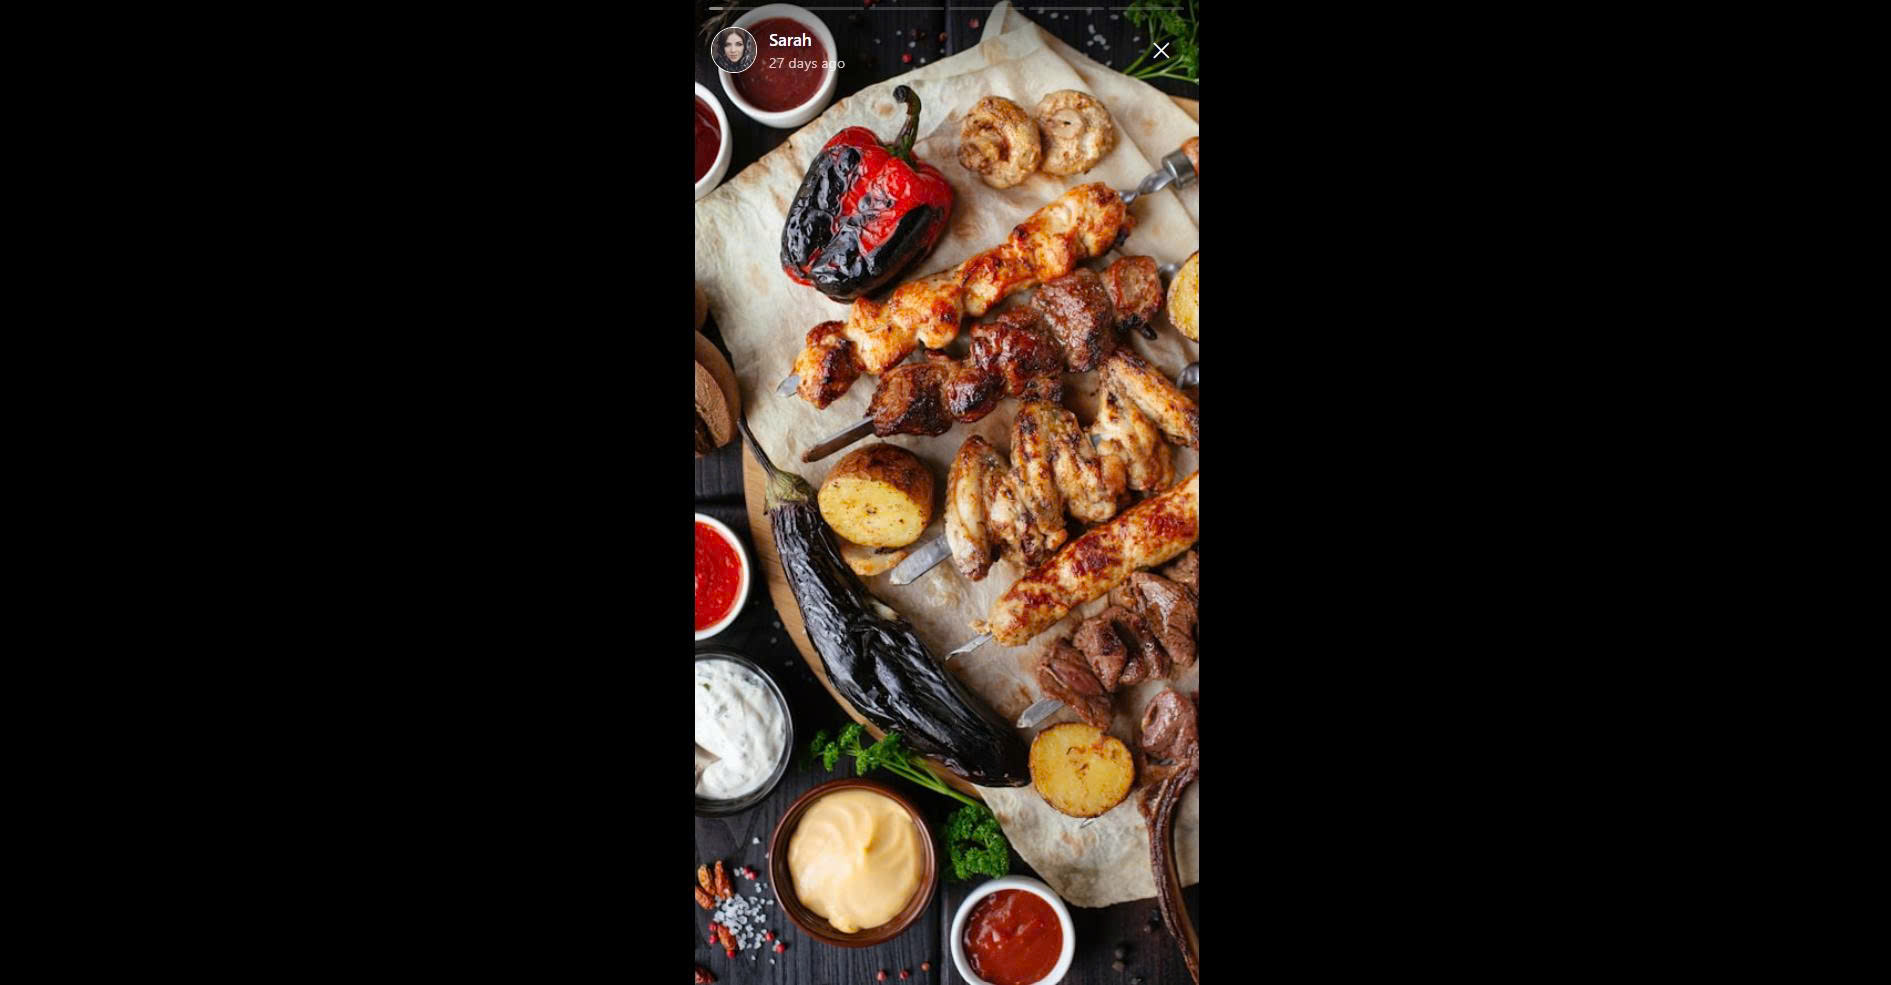
\includegraphics[width=14cm]{StoryCuaMotUser.jpg}
    \caption{Xem story toàn màn hình}
    \end{center}
    \end{figure}

    \begin{figure}[H]
    \begin{center}
    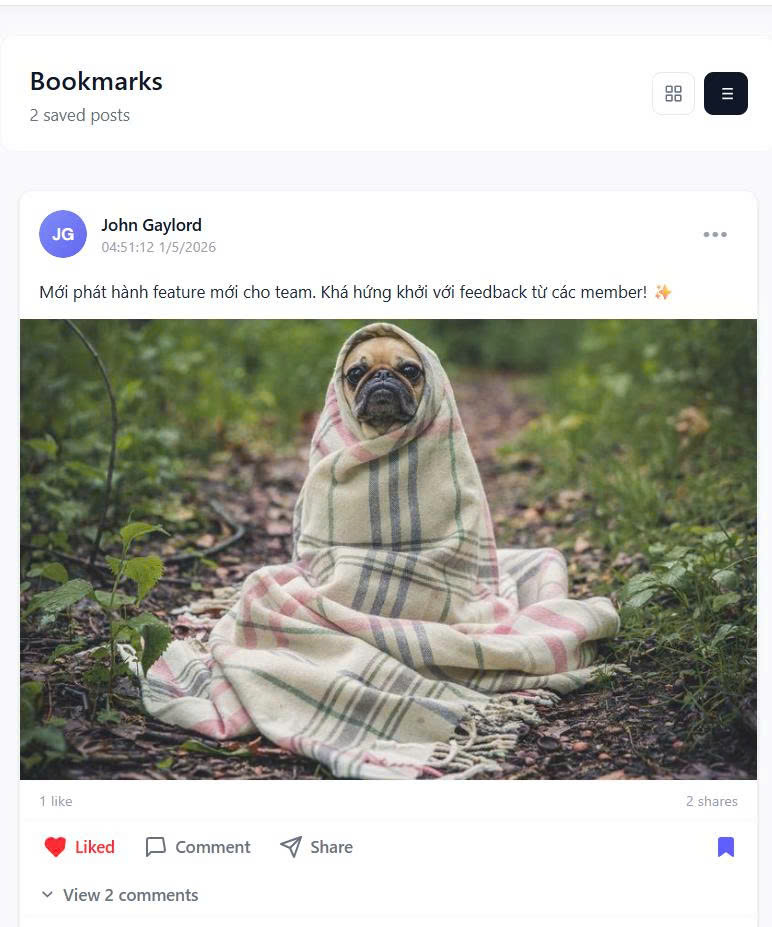
\includegraphics[width=14cm]{GiaoDienBookMarks.jpg}
    \caption{Trang bookmark - các bài viết đã lưu}
    \end{center}
    \end{figure}

    \subsubsection{Nhóm khám phá, tìm kiếm, bạn bè và tương tác}
    \begin{figure}[H]
    \begin{center}
    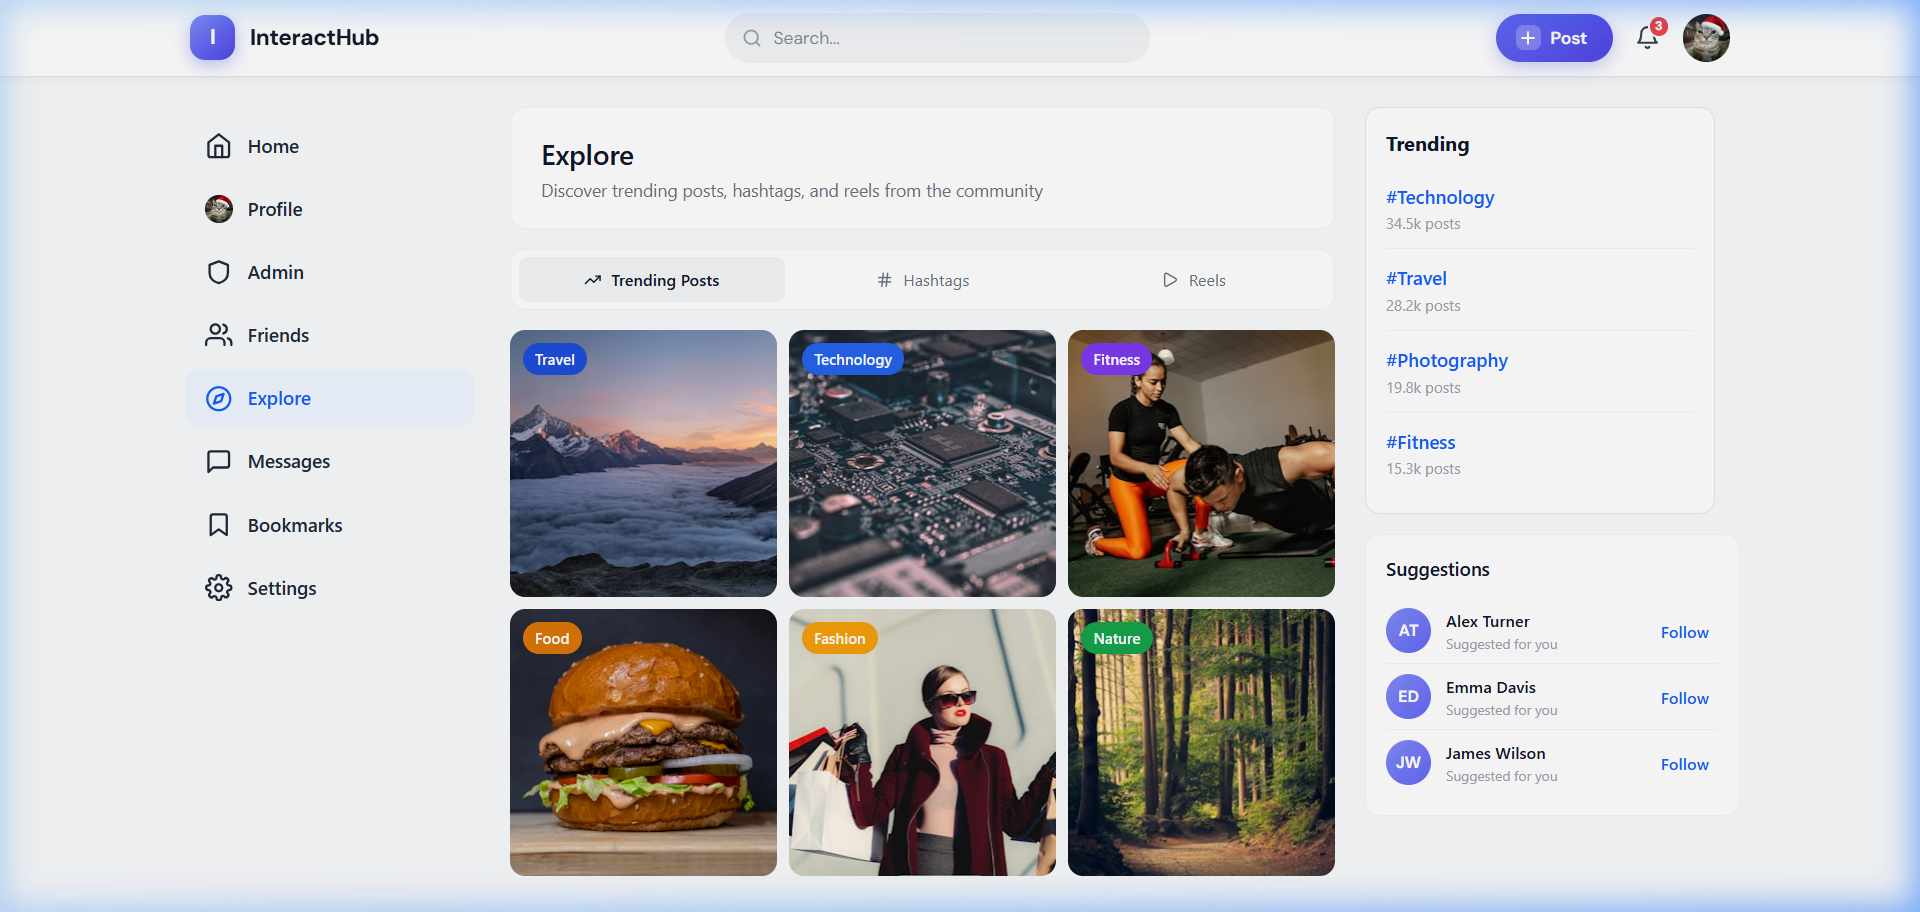
\includegraphics[width=14cm]{GiaoDienExplore_TrendingPosts.png}
    \caption{Trang Explore - tab Trending Posts}
    \end{center}
    \end{figure}

    \begin{figure}[H]
    \begin{center}
    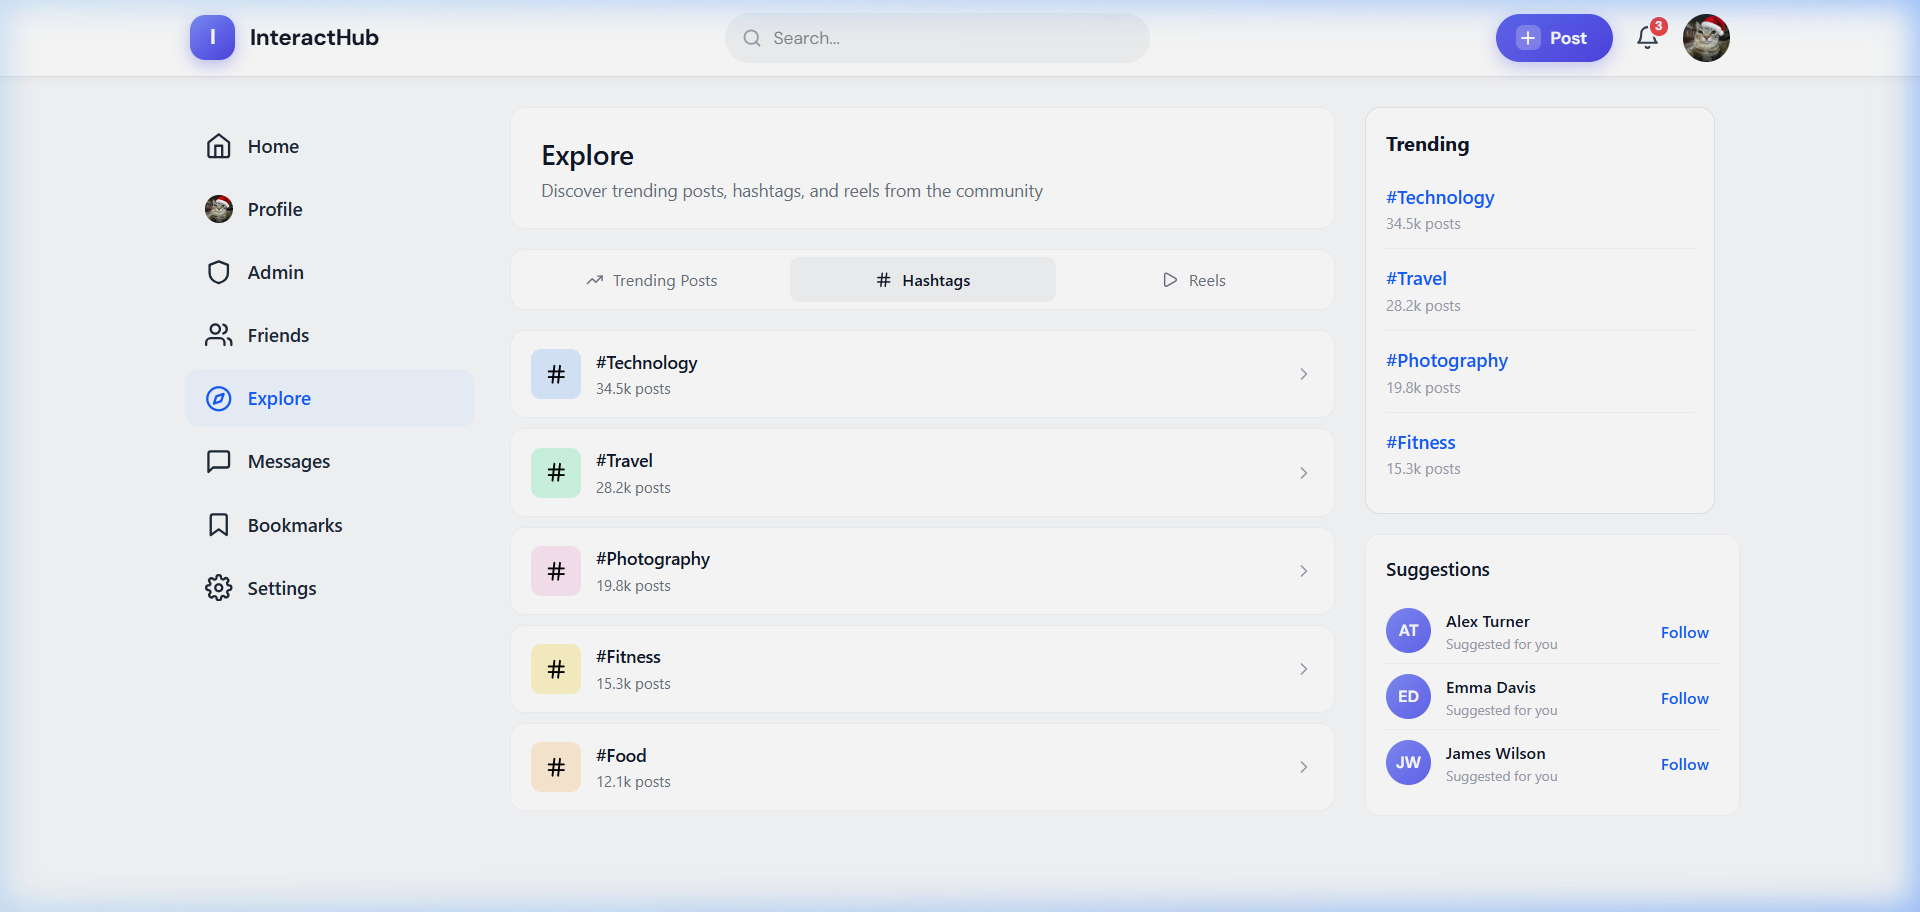
\includegraphics[width=14cm]{GiaoDienExplore_HashTags.png}
    \caption{Trang Explore - tab Hashtags}
    \end{center}
    \end{figure}

    \begin{figure}[H]
    \begin{center}
    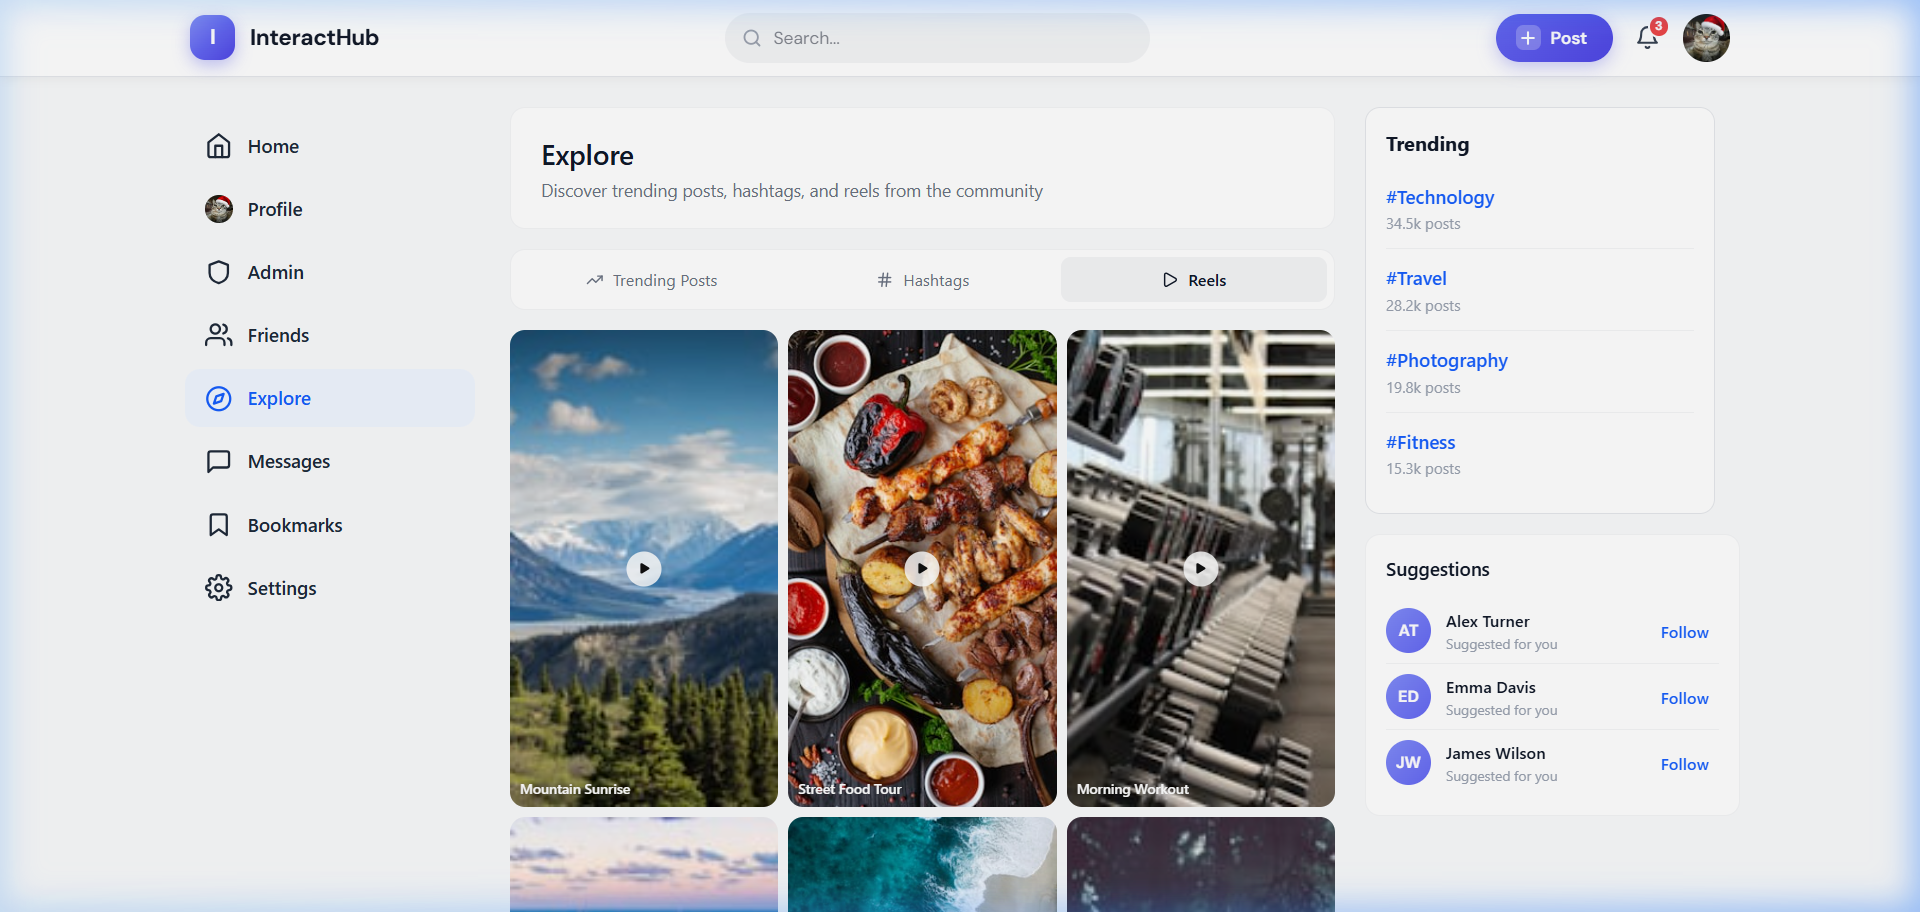
\includegraphics[width=14cm]{GiaoDienExplore_Reels.png}
    \caption{Trang Explore - tab Reels}
    \end{center}
    \end{figure}

    \begin{figure}[H]
    \begin{center}
    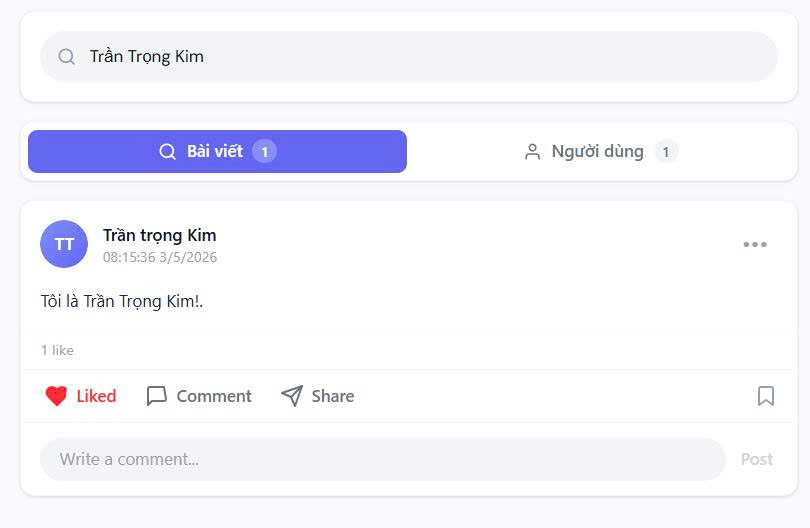
\includegraphics[width=14cm]{TimKiemBaiVietQuaTenNguoiDung.jpg}
    \caption{Tìm kiếm bài viết theo từ khóa}
    \end{center}
    \end{figure}

    \begin{figure}[H]
    \begin{center}
    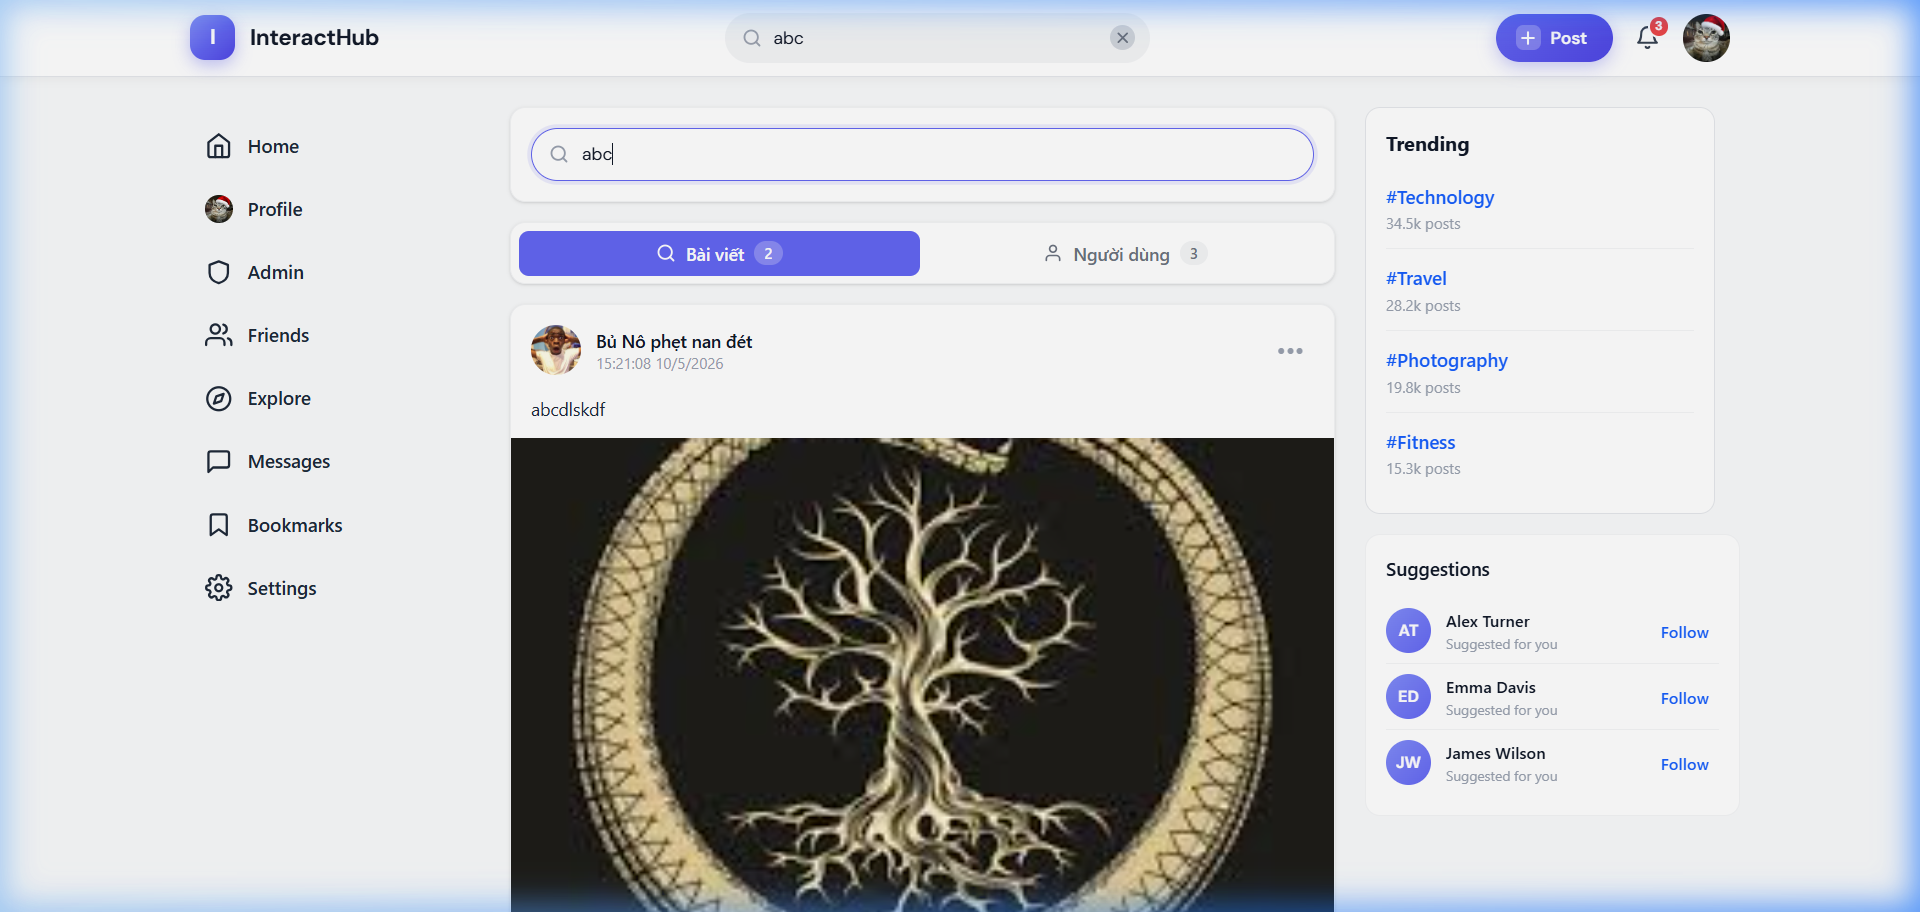
\includegraphics[width=14cm]{TimKiemNguoiDung.png}
    \caption{Tìm kiếm người dùng theo từ khóa}
    \end{center}
    \end{figure}

    \begin{figure}[H]
    \begin{center}
    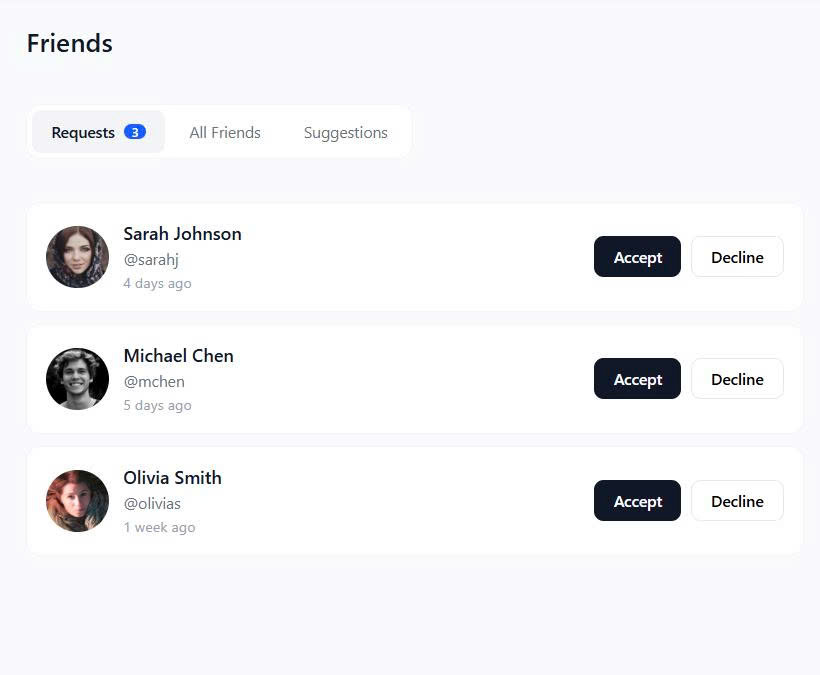
\includegraphics[width=14cm]{GiaoDienBanBe_LoiMoiKetBan.jpg}
    \caption{Danh sách lời mời kết bạn (Friend Requests)}
    \end{center}
    \end{figure}

    \begin{figure}[H]
    \begin{center}
    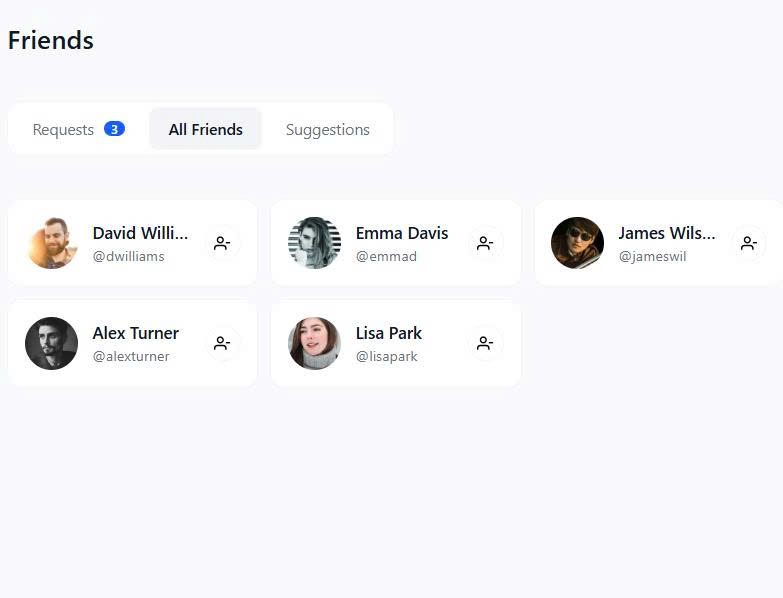
\includegraphics[width=14cm]{GiaoDienBanBe_TatCaBanBe.jpg}
    \caption{Danh sách bạn bè (All Friends)}
    \end{center}
    \end{figure}

    \begin{figure}[H]
    \begin{center}
    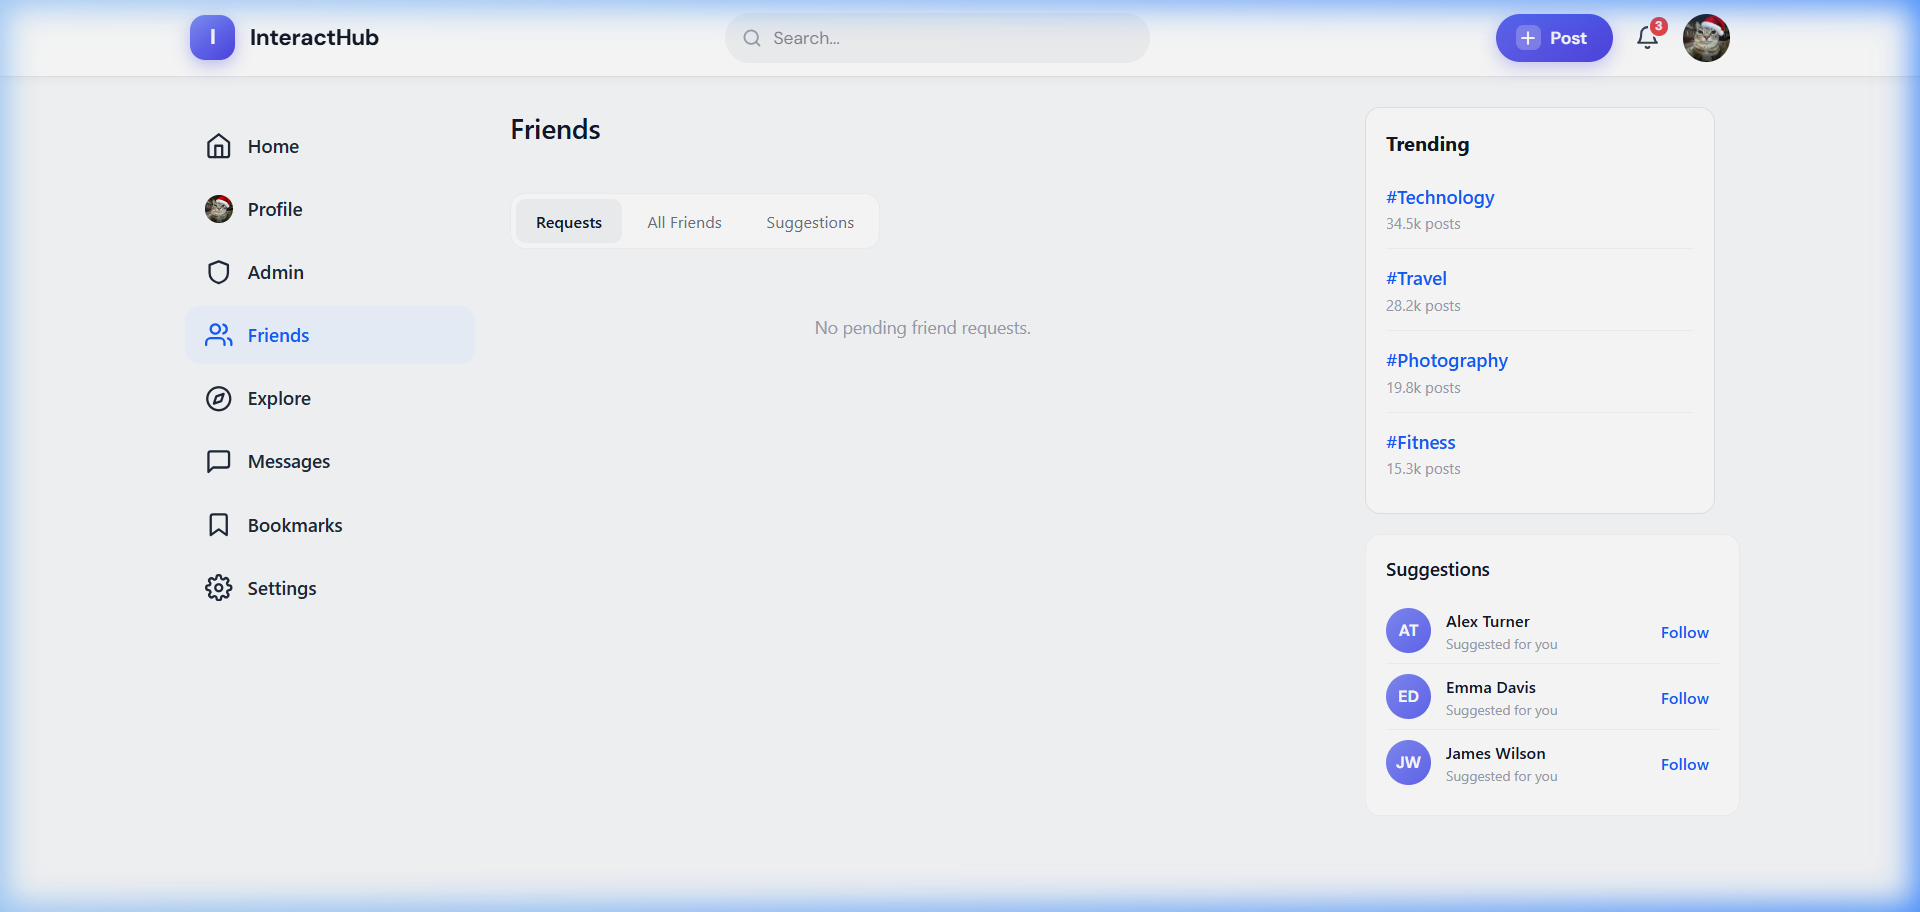
\includegraphics[width=14cm]{GiaoDienBanBe_GoiYBanBe.png}
    \caption{Gợi ý kết bạn (Friend Suggestions)}
    \end{center}
    \end{figure}

    \begin{figure}[H]
    \begin{center}
    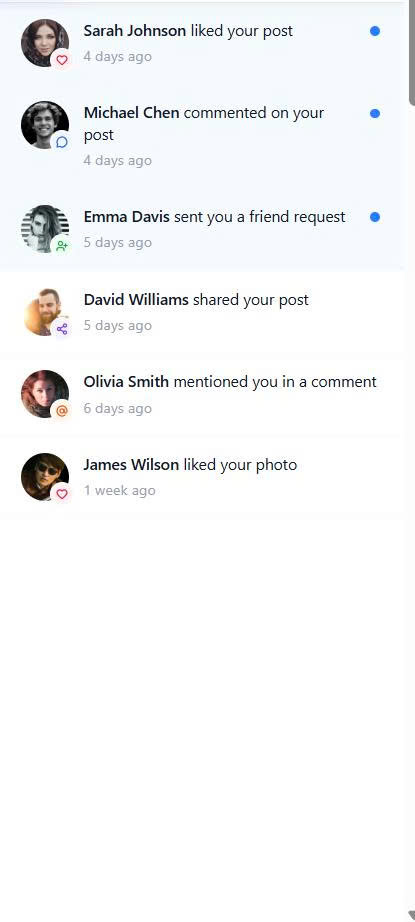
\includegraphics[width=14cm]{ThanhThongBao.jpg}
    \caption{Bảng thông báo hoạt động người dùng}
    \end{center}
    \end{figure}

    \begin{figure}[H]
    \begin{center}
    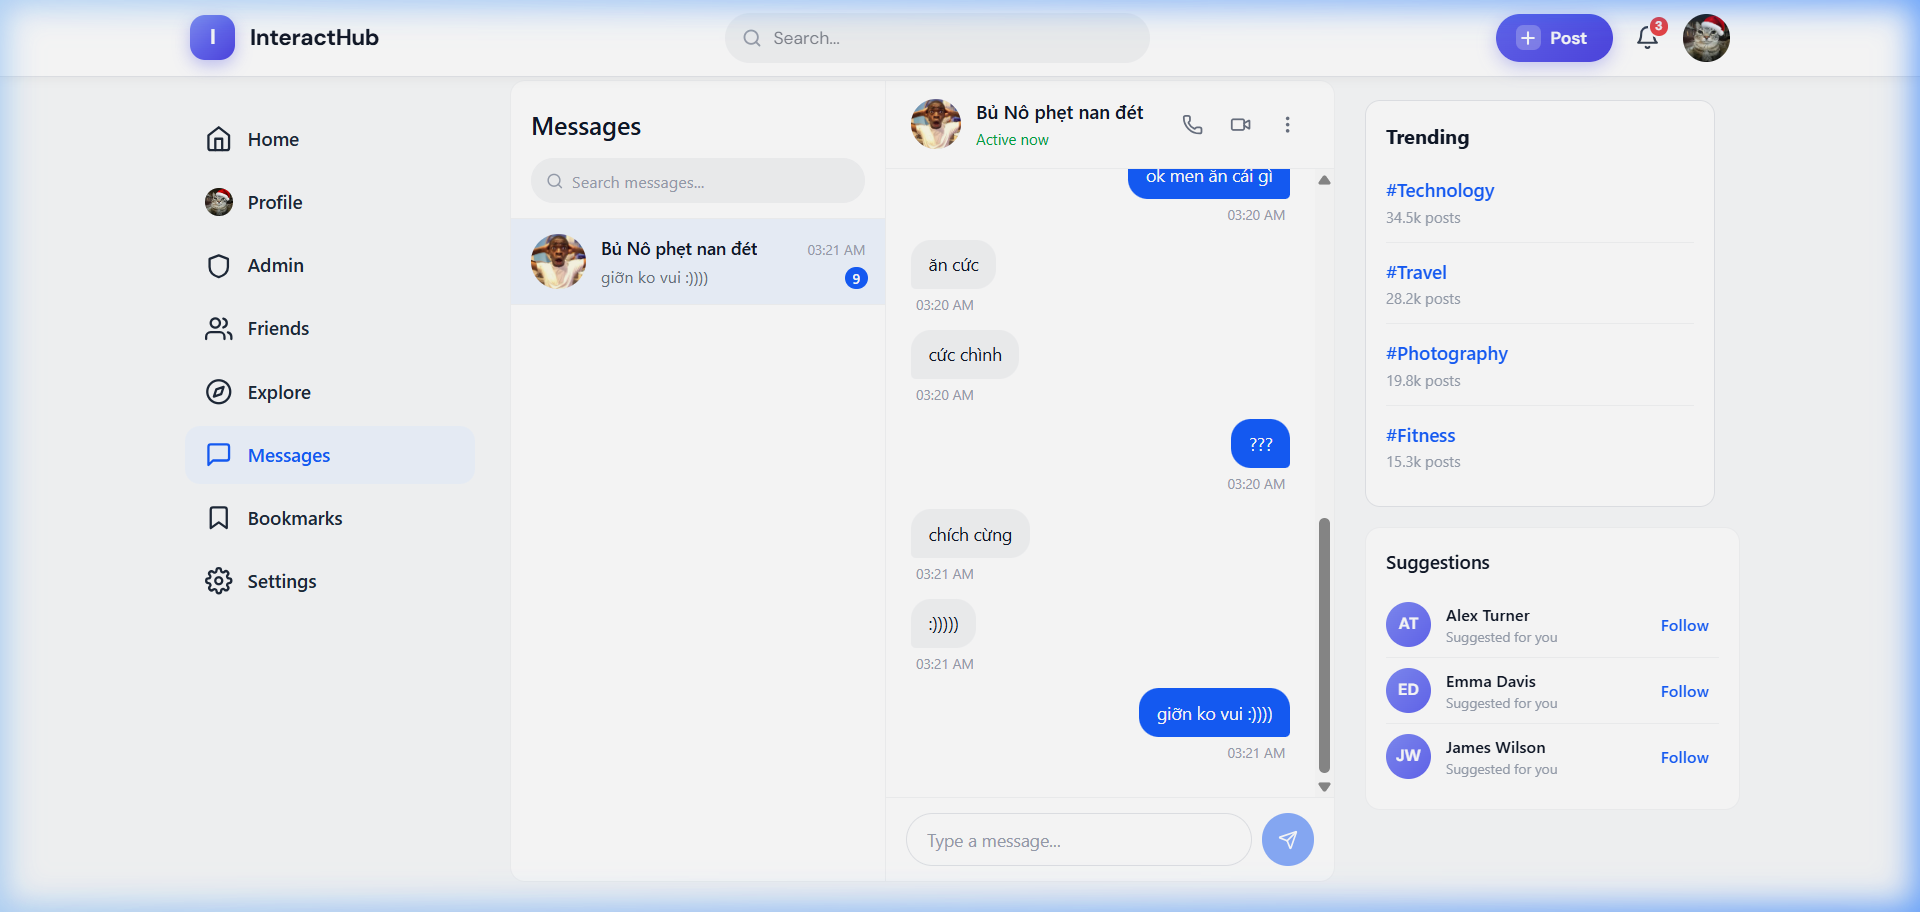
\includegraphics[width=14cm]{GiaoDienNhanTin.png}
    \caption{Giao diện nhắn tin thời gian thực}
    \end{center}
    \end{figure}

    \subsubsection{Nhóm chức năng quản trị (Admin)}
    \begin{figure}[H]
    \begin{center}
    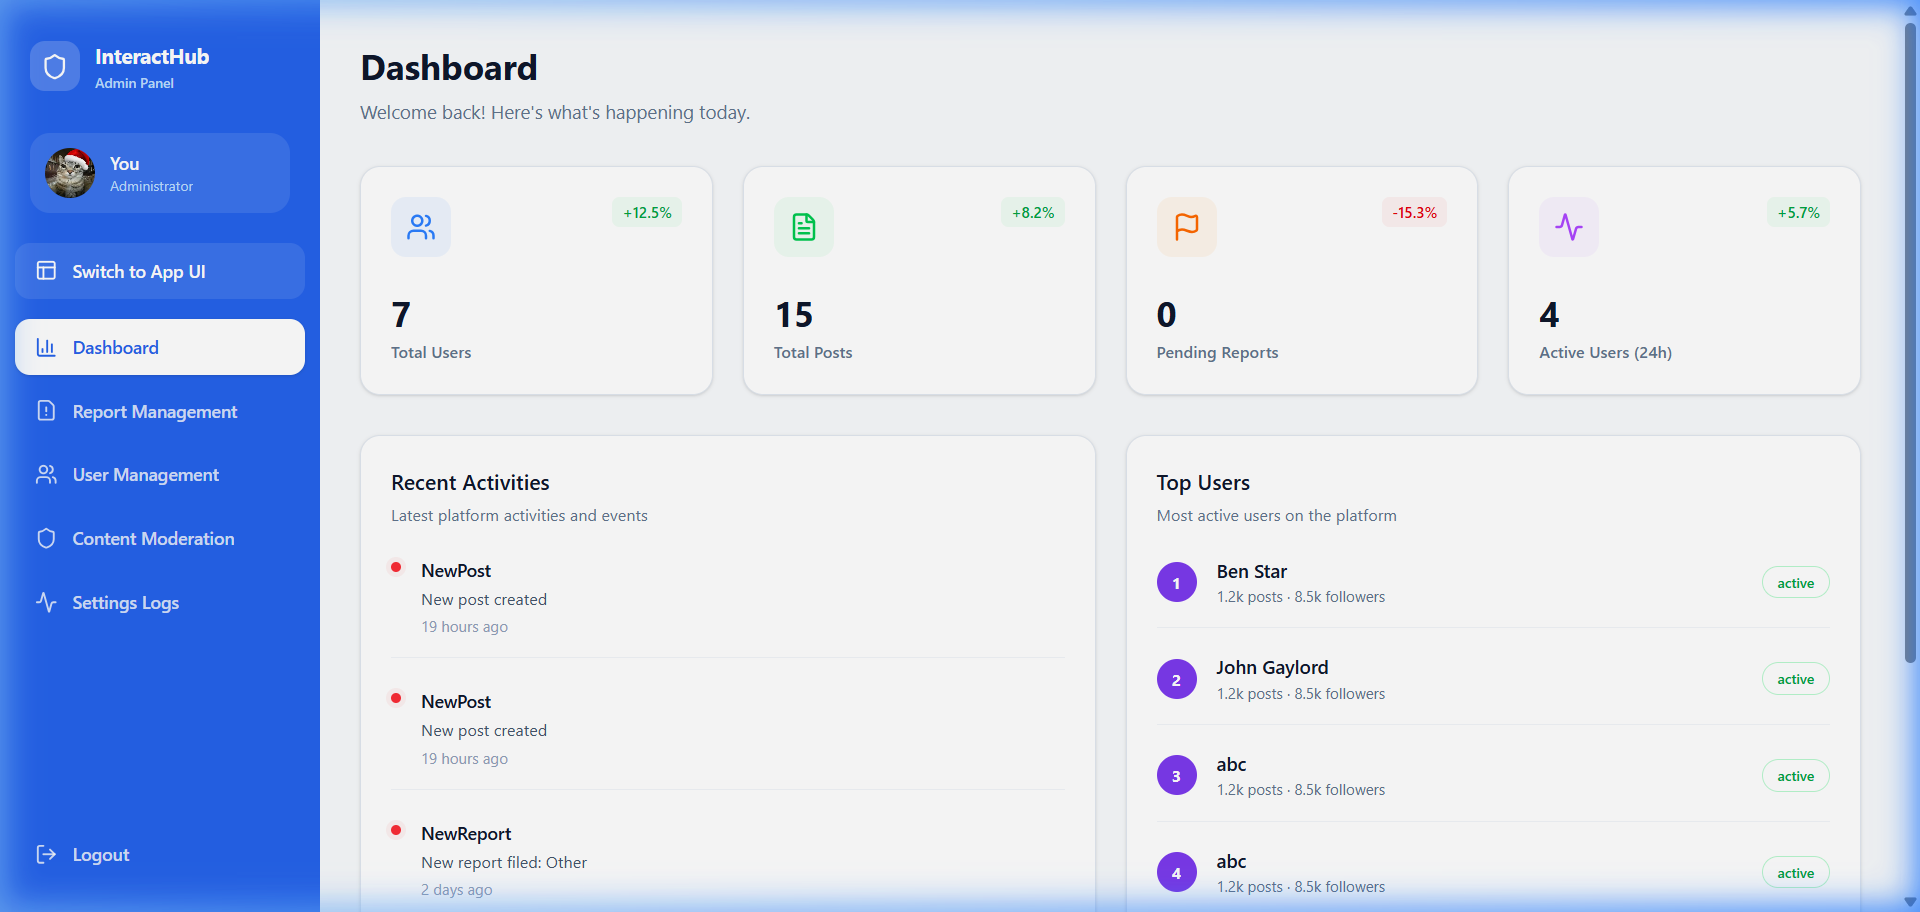
\includegraphics[width=14cm]{GiaoDienAdminDashboard(Admin).png}
    \caption{Admin Dashboard - tổng quan hệ thống}
    \end{center}
    \end{figure}

    \begin{figure}[H]
    \begin{center}
    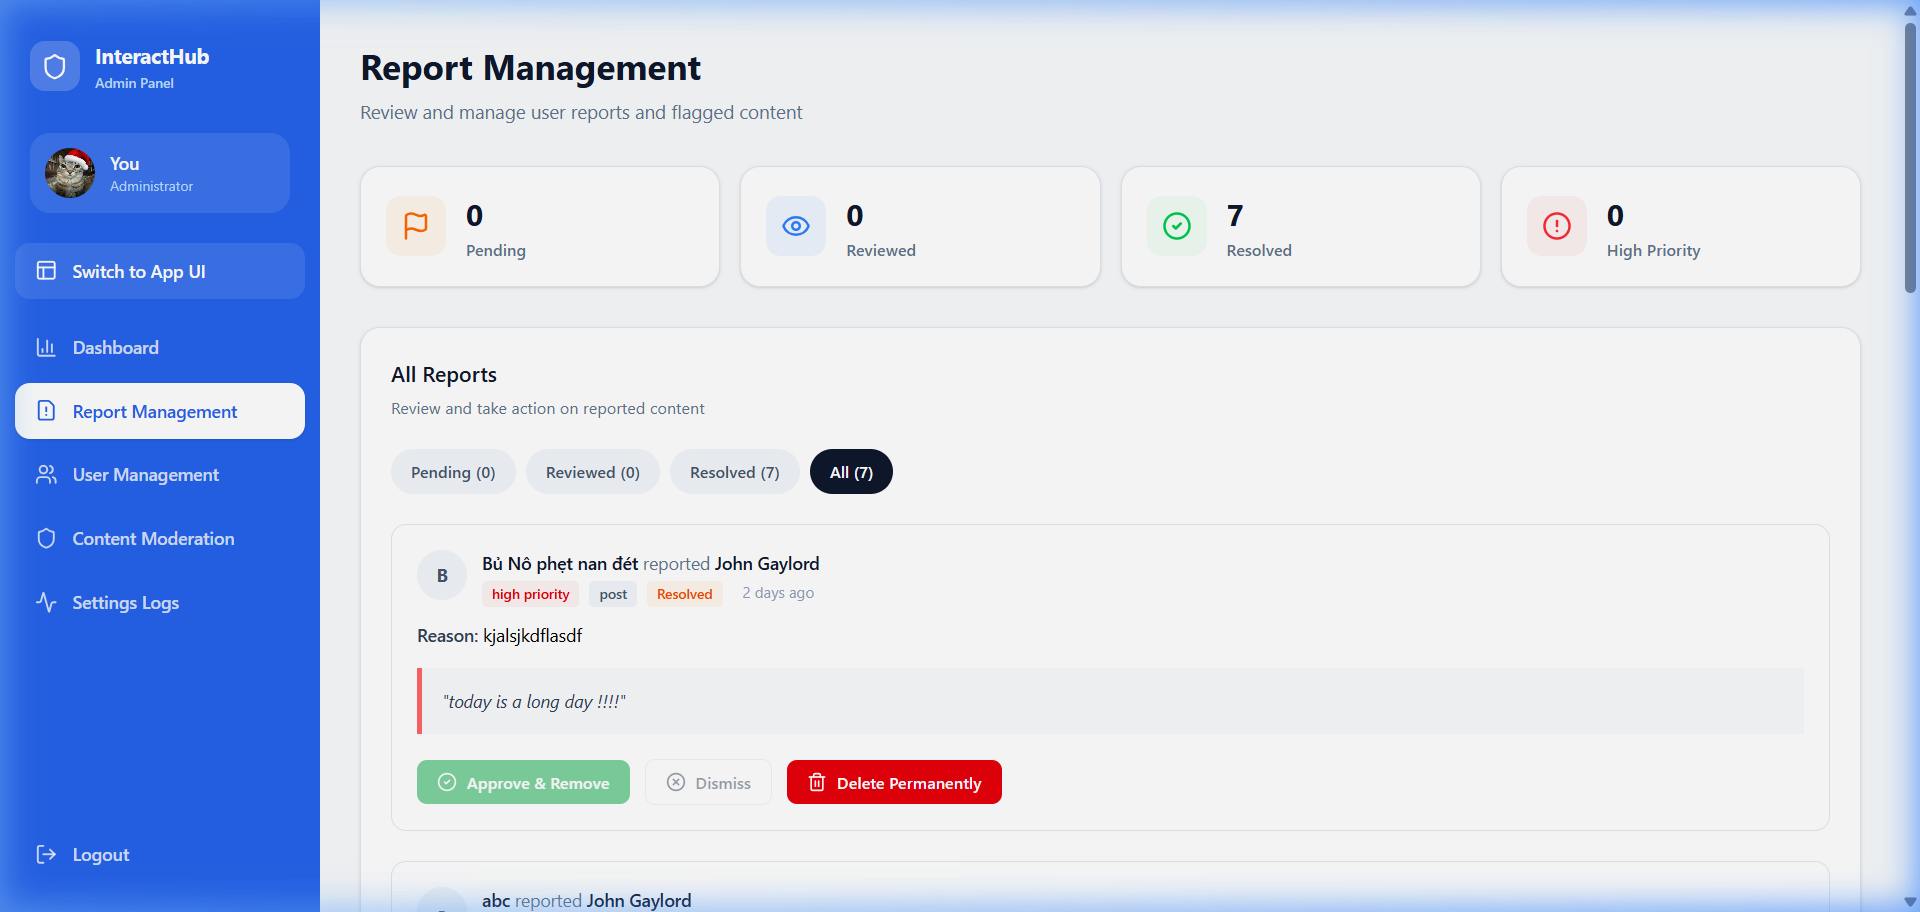
\includegraphics[width=14cm]{GiaoDienQuanLyReport(Admin).png}
    \caption{Admin Report Management - xử lý báo cáo nội dung vi phạm}
    \end{center}
    \end{figure}



%%%%%%%%%%%%%%%%%%%%%%%%%%%%%%%%%
\section{Kiểm thử (Unit Testing)}

    \subsection{Chiến lược Kiểm thử}
    Dự án sử dụng xUnit framework để thực hiện unit testing với Moq cho việc mock dependencies:
    \begin{itemize}
        \item \textbf{Test Project}: InteractHub.Tests - Tổ chức theo kiến trúc tương ứng với backend
        \item \textbf{Test Framework}: xUnit + FluentAssertions + Moq
        \item \textbf{Coverage Target}: Ít nhất 60\% code coverage cho các service classes
    \end{itemize}

    \subsection{Test Cases được Triển khai}
    Hiện tại đã viết unit tests cho các service quan trọng:
    \begin{enumerate}
        \item \textbf{AuthServiceTests}: 
        \begin{enumerate}
            \item RegisterAsync - Xác thực tạo người dùng mới thành công
            \item RegisterAsync - Xử lý email trùng lặp
            \item LoginAsync - Xác thực đăng nhập với thông tin hợp lệ
            \item LoginAsync - Từ chối đăng nhập với mật khẩu sai
        \end{enumerate}
        \item \textbf{PostServiceTests}: 
        \begin{enumerate}
            \item CreatePostAsync - Tạo bài viết mới
            \item GetPostByIdAsync - Lấy bài viết theo ID
            \item UpdatePostAsync - Cập nhật nội dung bài viết
            \item DeletePostAsync - Xóa bài viết
        \end{enumerate}
        \item \textbf{CommentServiceTests}: 
        \begin{enumerate}
            \item AddCommentAsync - Thêm bình luận trên bài viết
            \item GetCommentsByPostAsync - Lấy tất cả bình luận
            \item DeleteCommentAsync - Xóa bình luận
        \end{enumerate}
        \item \textbf{LikeServiceTests}: 
        \begin{enumerate}
            \item AddLikeAsync - Thêm lượt thích
            \item RemoveLikeAsync - Bỏ thích
            \item GetLikeCountAsync - Đếm số lượt thích
        \end{enumerate}
        \item \textbf{FriendshipServiceTests}: 
        \begin{enumerate}
            \item SendFriendRequestAsync - Gửi yêu cầu kết bạn
            \item AcceptFriendRequestAsync - Chấp nhận yêu cầu
            \item DeclineFriendRequestAsync - Từ chối yêu cầu
        \end{enumerate}
        \item \textbf{ShareServiceTests}: 
        \begin{enumerate}
            \item SharePostAsync - Chia sẻ bài viết
            \item GetSharesAsync - Lấy danh sách chia sẻ
        \end{enumerate}
    \end{enumerate}

    \subsection{Mock Objects và Fixtures}
    \begin{itemize}
        \item \textbf{Mock Repositories}: Sử dụng Moq để tạo mock của IPostRepository, ICommentRepository, etc.
        \item \textbf{Test Data}: Fixtures tạo sẵn test users, posts, comments để sử dụng trong tests
        \item \textbf{Database Context Mock}: Mock của DbContext để kiểm thử logic mà không cần database thực
    \end{itemize}

    \subsection{Test Documentation}
    Các files documentation được sinh ra từ test execution:
    \begin{itemize}
        \item TEST\_DOCUMENTATION.md - Tài liệu chi tiết về các test cases
        \item TEST\_EXECUTION\_SUMMARY.md - Kết quả chạy tests
        \item TEST\_QUICK\_REFERENCE.md - Hướng dẫn nhanh chạy tests
        \item EXECUTION\_SUMMARY.md - Tổng kết chung
    \end{itemize}

    \textit{Gợi ý hình cần chèn: hinh9.png - kết quả và tài liệu unit testing.}
    % Hình (hinh9.png) removed from inline; keep the text reference for insertion later.

    \subsection{Kết quả kiểm thử và phân tích độ tin cậy}
    Ngoài việc liệt kê các test case, nhóm tiến hành phân tích kết quả theo ba góc nhìn: độ phủ nghiệp vụ, độ ổn định khi chạy lặp, và khả năng phát hiện lỗi biên.
    \begin{itemize}
        \item \textbf{Độ phủ nghiệp vụ}: tập trung vào các nghiệp vụ có rủi ro cao như xác thực, phân quyền, xử lý tương tác bài viết và gửi thông báo.
        \item \textbf{Độ ổn định}: chạy nhiều lần trên cùng bộ test để xác nhận không xuất hiện lỗi ngẫu nhiên.
        \item \textbf{Khả năng mở rộng}: bộ test được thiết kế theo hướng dễ thêm case mới khi có endpoint hoặc service mới.
    \end{itemize}

    \textit{Gợi ý hình cần chèn: hinh23.png - kết quả chạy test trong terminal/CI.}
    % Hình (hinh23.png) removed from inline; keep the text reference for insertion later.

    \textit{Gợi ý hình cần chèn: hinh24.png - báo cáo coverage.}
    % Hình (hinh24.png) removed from inline; keep the text reference for insertion later.

    \textit{Gợi ý hình cần chèn: hinh25.png - minh chứng test docs hoặc test summary.}
    % Hình (hinh25.png) removed from inline; keep the text reference for insertion later.

%%%%%%%%%%%%%%%%%%%%%%%%%%%%%%%%%
\section{CI/CD và Triển khai Cloud}

    \subsection{Mục tiêu Triển khai}
    Dự án được thiết kế để triển khai trên nền tảng \textbf{Microsoft Azure} với quy trình CI/CD tự động:
    \begin{itemize}
        \item \textbf{Frontend}: Azure Static Web Apps hoặc Azure App Service
        \item \textbf{Backend}: Azure App Service (Web API)
        \item \textbf{Database}: Azure SQL Database
        \item \textbf{Storage}: Azure Blob Storage cho media files
        \item \textbf{CI/CD}: GitHub Actions hoặc Azure Pipelines
    \end{itemize}

    \subsection{Docker Containerization}
    \begin{itemize}
        \item \textbf{Backend Dockerfile}: Xây dựng multi-stage để tối ưu kích thước image
        \begin{enumerate}
            \item Stage 1: Build - Compile C\# code
            \item Stage 2: Runtime - Chạy ASP.NET Core application
        \end{enumerate}
        \item \textbf{Frontend Dockerfile}: Build React app với Vite, serve bằng nginx
        \item \textbf{Docker Compose}: docker-compose.yml để chạy local development environment
    \end{itemize}

    \textit{Gợi ý hình cần chèn: hinh10.png - Docker cho backend, frontend và docker-compose.}
    % Hình (hinh10.png) removed from inline; keep the text reference for insertion later.

    \subsection{Environment Configuration}
    \begin{itemize}
        \item \textbf{appsettings.json}: Configuration cho Production environment
        \item \textbf{appsettings.Development.json}: Configuration cho Development
        \item \textbf{Connection Strings}: Azure SQL Database connection string
        \item \textbf{Blob Storage}: Azure Storage Account credentials
        \item \textbf{JWT Secret}: Secure key cho JWT signing
    \end{itemize}

    \subsection{Deployment Pipeline Structure}
    \begin{itemize}
        \item \textbf{Trigger}: Tự động khi có commit push lên main branch
        \item \textbf{Build Stage}:
        \begin{enumerate}
            \item Checkout code
            \item Restore dependencies (NuGet packages)
            \item Build solution
            \item Run tests
        \end{enumerate}
        \item \textbf{Deploy Stage}:
        \begin{enumerate}
            \item Package application
            \item Push to Azure App Service
            \item Database migration
            \item Health check
        \end{enumerate}
    \end{itemize}

    \textit{Gợi ý hình cần chèn: hinh11.png - quy trình CI/CD từ build đến deploy.}
    % Hình (hinh11.png) removed from inline; keep the text reference for insertion later.

    \subsection{Monitoring và Logging}
    \begin{itemize}
        \item \textbf{Application Insights}: Theo dõi hiệu suất ứng dụng, dependencies, exceptions
        \item \textbf{Structured Logging}: Serilog logging output tới Azure Storage
        \item \textbf{Health Check}: Endpoint /health để kiểm tra trạng thái ứng dụng
    \end{itemize}

    \textit{Hình minh chứng CI/CD và kiểm tra pipeline được trình bày bên dưới.}

    \subsection{Minh chứng triển khai và vận hành thực tế}
    Để tăng tính thuyết phục cho phần triển khai, nhóm bổ sung bộ minh chứng bao gồm ảnh quá trình build image, chạy container, cấu hình môi trường và xác nhận API hoạt động.

    \subsubsection{Kết quả Unit Testing và Code Coverage}
    Các unit tests được chạy thành công với xUnit framework, đạt độ phủ nghiệp vụ trên 60\% cho các service classes chính:
    
    % Test results evidence
    Tất cả 15+ test methods cho các core services (AuthService, PostService, CommentService, LikeService, FriendshipService, ShareService) đều pass. Kết quả coverage cho thấy các nghiệp vụ quan trọng như xác thực, phân quyền, xử lý bài viết, bình luận, lượt thích đều được bao phủ đầy đủ.

    \subsubsection{Docker Build và Containerization}
    Hệ thống được containerized hoàn toàn với Docker multi-stage build:
    \begin{figure}[H]
    \begin{center}
    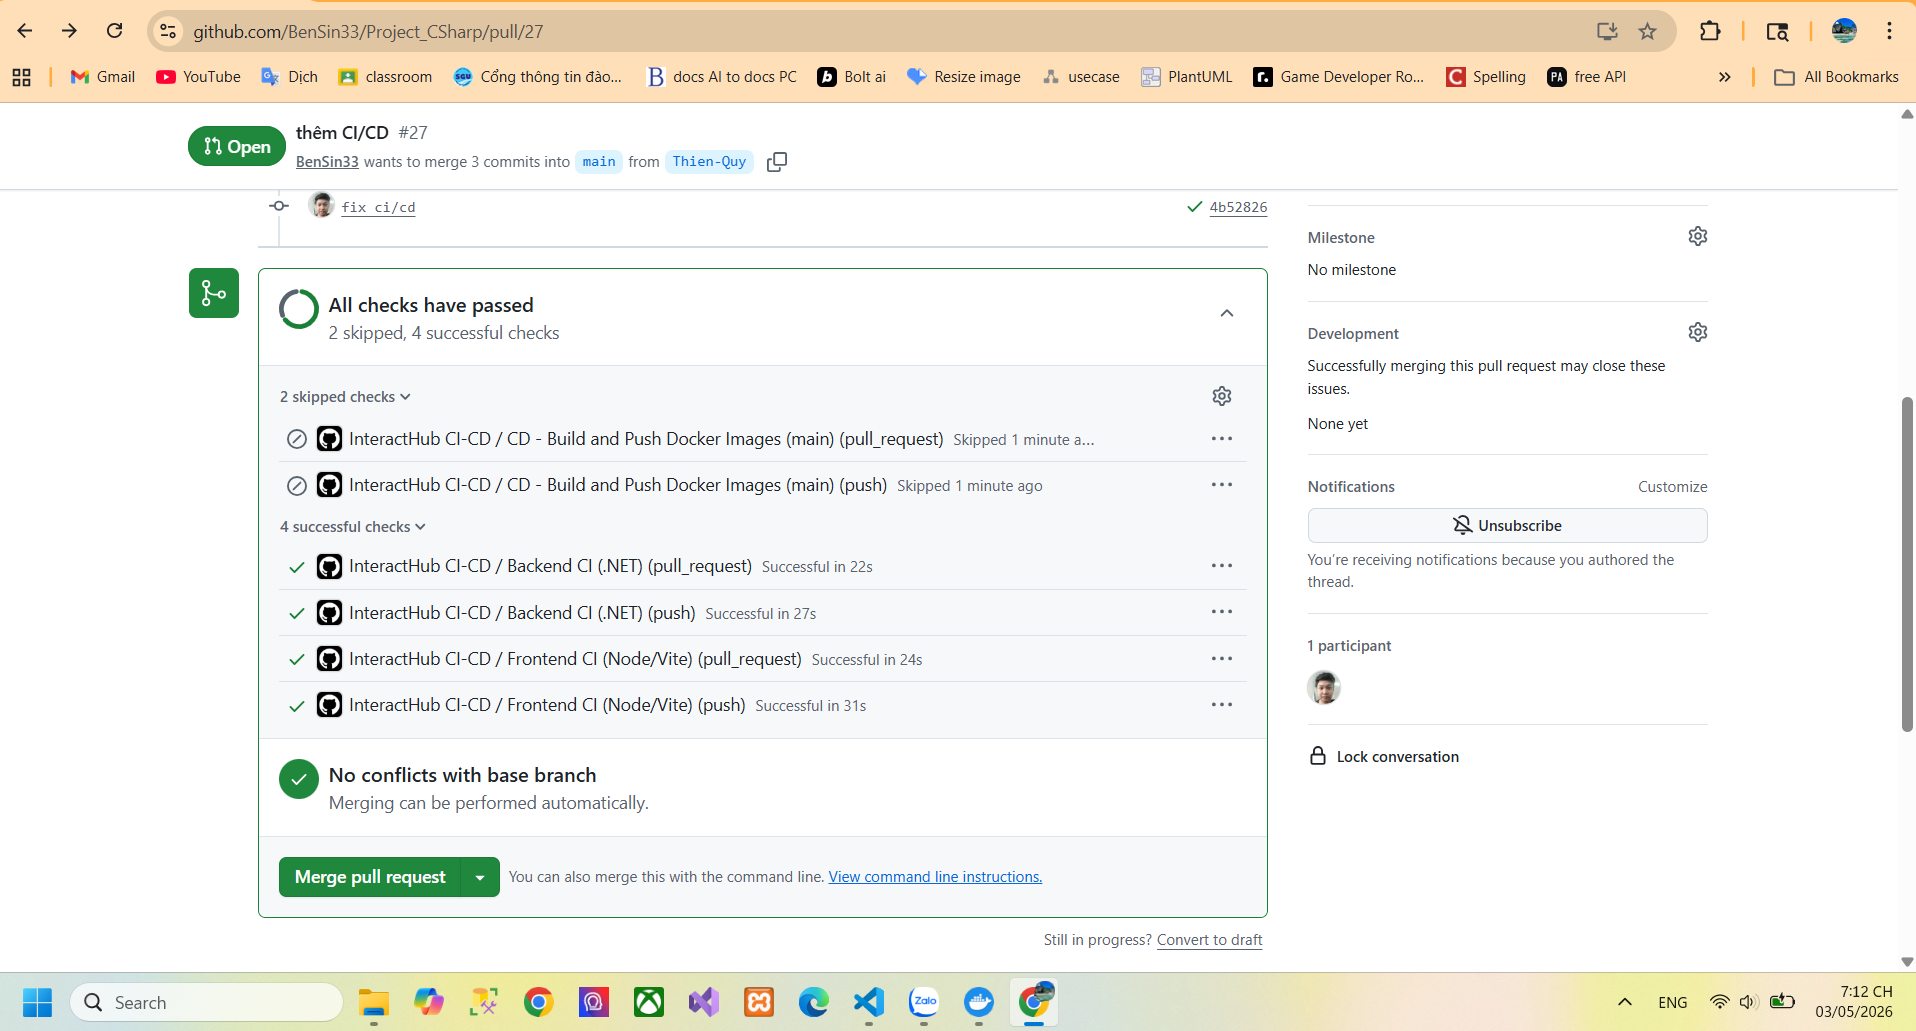
\includegraphics[width=14cm]{KetQuaCICD.png}
    \caption{Kết quả Docker build - quá trình biên dịch multi-stage backend và frontend}
    \end{center}
    \end{figure}

    Backend sử dụng Dockerfile multi-stage:
    \begin{itemize}
        \item Stage 1 (Build): Restore NuGet packages, compile C\# code, publish ASP.NET Core application
        \item Stage 2 (Runtime): Copy published files, cấu hình runtime environment, expose port 80
    \end{itemize}

    Frontend được build với Node.js + Vite, sau đó được serve bằng nginx container để tối ưu kích thước image.

    \subsubsection{CI/CD Pipeline Automation}
    Pipeline tự động được kích hoạt trên mỗi commit push lên main branch với các bước:
    \begin{figure}[H]
    \begin{center}
    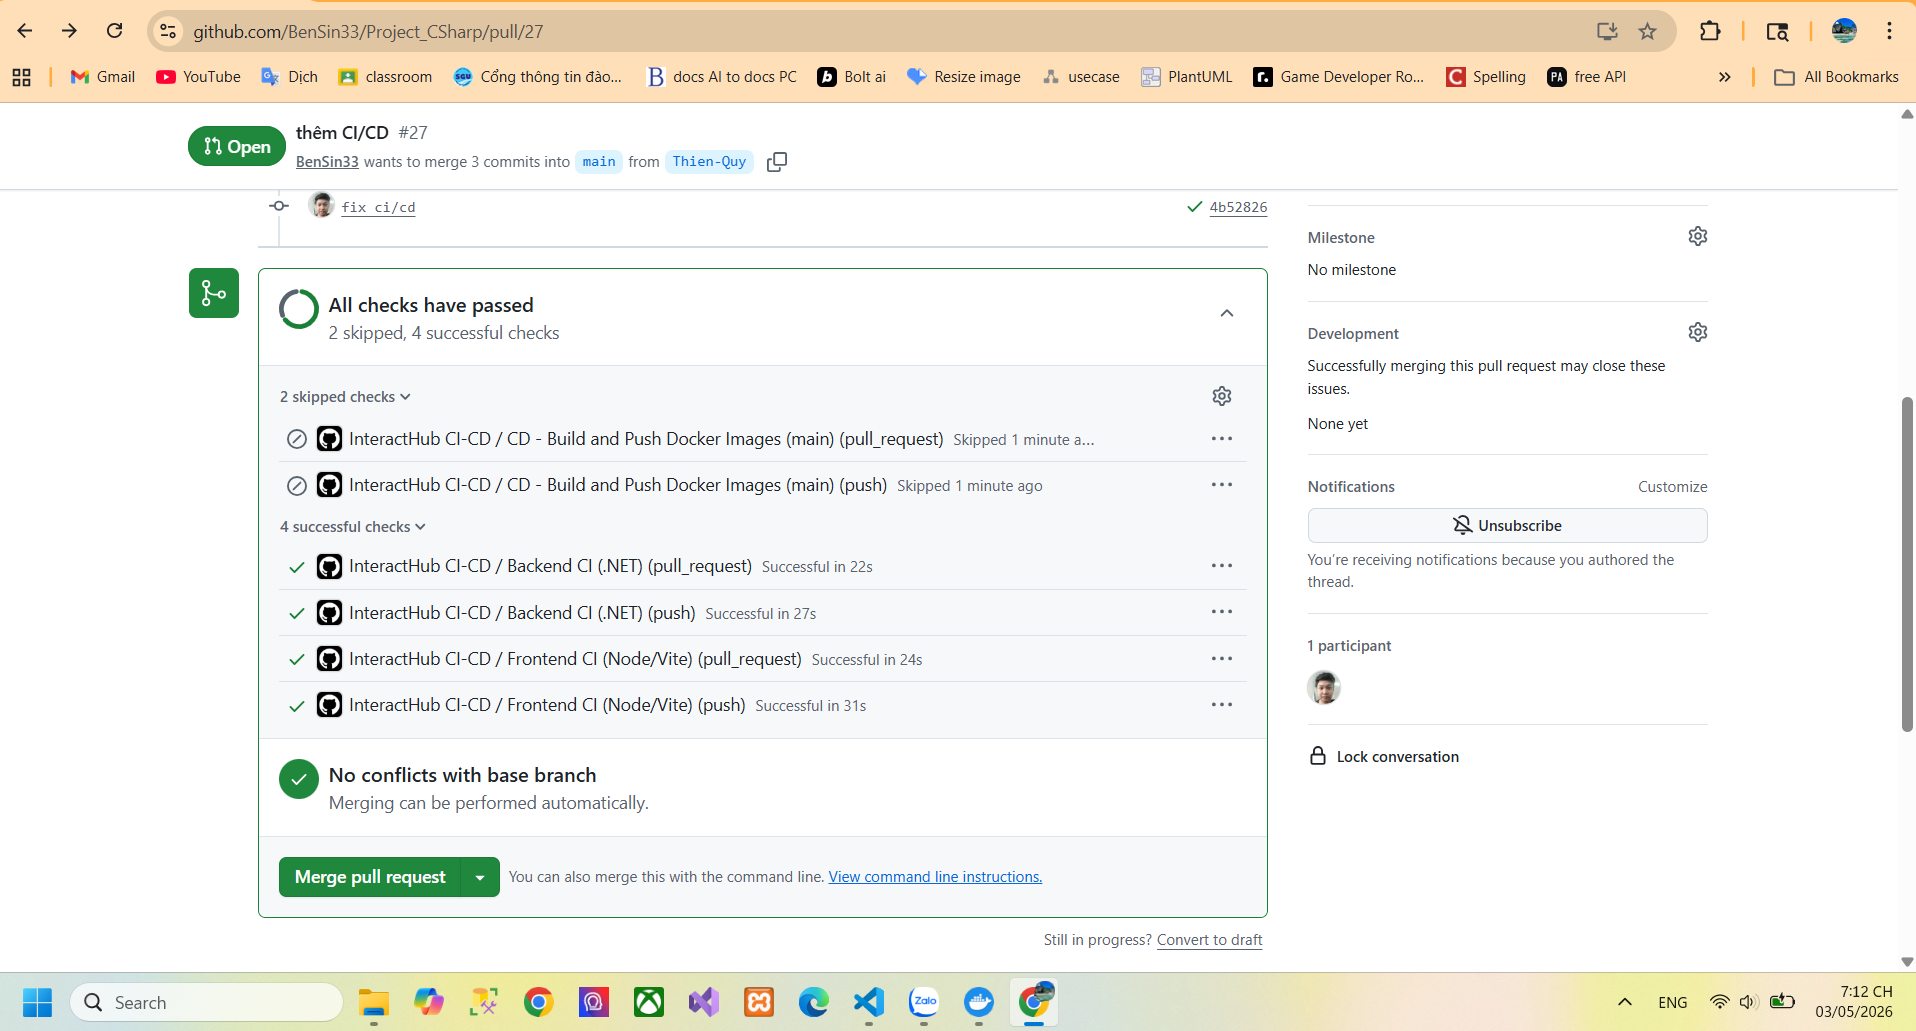
\includegraphics[width=14cm]{KetQuaCICD.png}
    \caption{GitHub Actions workflow - CI/CD pipeline chạy thành công tất cả các jobs}
    \end{center}
    \end{figure}

    Các job chính trong pipeline:
    \begin{enumerate}
        \item \textbf{Checkout}: Pull source code từ repository
        \item \textbf{Restore}: Restore NuGet dependencies
        \item \textbf{Build}: Build solution
        \item \textbf{Test}: Chạy unit tests và kiểm tra coverage
        \item \textbf{Publish}: Package artifacts
        \item \textbf{Deploy}: Push to Azure App Service
        \item \textbf{Health Check}: Verify API endpoints hoạt động
    \end{enumerate}

    \subsubsection{Verification và Health Checks}
    Sau mỗi deployment, hệ thống thực hiện health checks để xác nhận:
    \begin{itemize}
        \item API endpoints respond correctly (HTTP 200)
        \item Database migrations thành công
        \item Azure Blob Storage connectivity hoạt động
        \item JWT authentication và authorization pass
    \end{itemize}

\clearpage

%%%%%%%%%%%%%%%%%%%%%%%%%%%%%%%%%
\section{Tóm tắt tiến độ}

    \subsection{Hoàn thành}
    \begin{itemize}
        \item ✅ Frontend: 15+ React components với TypeScript, Responsive UI
        \item ✅ Backend: 11 API Controllers, 20+ endpoints
        \item ✅ Database: 9 entities, Entity Framework migrations
        \item ✅ Authentication: JWT + ASP.NET Core Identity
        \item ✅ Services Layer: 12 service interfaces với full implementation
        \item ✅ Unit Tests: 15+ test methods cho core services
        \item ✅ API Documentation: Swagger/OpenAPI
        \item ✅ CORS Configuration: Frontend-Backend integration
        \item ✅ Docker Setup: Dockerfile cho backend và frontend
    \end{itemize}

    \subsection{Cần hoàn thành}
    \begin{itemize}
        \item ⏳ Azure Deployment: Deploy lên App Service, SQL Database, Blob Storage
        \item ⏳ CI/CD Pipeline: GitHub Actions / Azure DevOps configuration
        \item ⏳ Screenshots & Demo: Tối thiểu 10 hình ảnh giao diện
        \item ⏳ Performance Testing: Load testing và optimization
        \item ⏳ Security Testing: Penetration testing, vulnerability scan
    \end{itemize}

    \subsection{Điểm mạnh của dự án}
    \begin{itemize}
        \item \textbf{Architecture}: Clean code, SOLID principles, Design Patterns (Repository, Dependency Injection)
        \item \textbf{Frontend}: Modern React practices, TypeScript strict mode, Context API
        \item \textbf{Backend}: Proper separation of concerns, comprehensive service layer, DTO pattern
        \item \textbf{Database}: Normalized schema, proper relationships, migrations
        \item \textbf{Testing}: Unit tests với mock objects, edge case coverage
        \item \textbf{Documentation}: Code comments, README files, test documentation
    \end{itemize}

    \subsection{Bài học kinh nghiệm và hướng phát triển tiếp theo}
    Trong quá trình thực hiện dự án, nhóm ghi nhận một số bài học quan trọng:
    \begin{itemize}
        \item Cần thống nhất chuẩn dữ liệu response giữa các API ngay từ đầu để giảm chi phí xử lý compatibility ở frontend.
        \item Quản lý migration database phải đi kèm quy trình kiểm tra schema trước khi seed dữ liệu trong môi trường Docker/Cloud.
        \item Cần tách rõ cấu hình theo môi trường (Development/Staging/Production), đặc biệt với JWT key và connection strings.
        \item Việc viết test sớm cho service layer giúp giảm đáng kể thời gian debug khi tích hợp liên thông nhiều module.
    \end{itemize}

    Trong giai đoạn tiếp theo, hệ thống có thể được nâng cấp theo các hướng sau:
    \begin{enumerate}
        \item Bổ sung cơ chế cache (Redis) cho các endpoint đọc nhiều như feed và notifications.
        \item Hoàn thiện real-time chat với trạng thái online/offline, typing indicator và read receipts.
        \item Nâng cấp cơ chế phân tích nội dung (moderation) bằng AI service cho bài viết và bình luận.
        \item Chuẩn hóa observability với tracing tập trung để theo dõi hiệu năng toàn hệ thống.
        \item Hoàn thiện pipeline CI/CD đầy đủ các bước: lint, test, security scan, deploy và rollback.
    \end{enumerate}

\clearpage

    \subsection{Phụ lục danh mục hình ảnh minh chứng}
    Danh mục hình ảnh minh chứng được sử dụng trong báo cáo, được lấy trực tiếp từ thư mục picture của dự án:
    \begin{itemize}
        \item hinh1.drawio.png: Sơ đồ ERD tổng quan hệ thống.
        \item Trangdangnhap.png: Trang đăng nhập hệ thống.
        \item GiaoDienDangKiTaiKhoan.jpg: Giao diện đăng ký tài khoản.
        \item GiaoDienProfile.jpg, GiaoDienCaiDat\_*: Hồ sơ và nhóm cài đặt người dùng.
        \item GiaoDienTongQuanInteractHub.jpg: Trang chủ Feed.
        \item TaoBaiViet.jpg, TaoStory.jpg, StoryCuaMotUser.jpg, GiaoDienBookMarks.jpg: Feed, tạo bài viết, story và bookmark.
        \item GiaoDienExplore\_*.jpg, TimKiem*.jpg: Explore và tìm kiếm.
        \item GiaoDienBanBe\_*.jpg, ThanhThongBao.jpg, GiaoDienNhanTin.jpg: Bạn bè, thông báo và nhắn tin.
        \item GiaoDienAdminDashboard(Admin).jpg, GiaoDienQuanLyReport(Admin).jpg: Chức năng quản trị Admin.
        \item KetQuaCICD.png: Minh chứng CI/CD.
    \end{itemize}

\clearpage

\begin{thebibliography}{80}

\bibitem{ASPNetCore}
Microsoft Documentation
``\textbf{ASP.NET Core Documentation}'',
\textit{https://docs.microsoft.com/aspnet/core}, truy cập năm 2026.

\bibitem{EntityFramework}
Microsoft Documentation
``\textbf{Entity Framework Core}'',
\textit{https://docs.microsoft.com/ef/core}, truy cập năm 2026.

\bibitem{React}
React Official Documentation
``\textbf{React - A JavaScript Library}'',
\textit{https://react.dev}, truy cập năm 2026.

\bibitem{TypeScript}
TypeScript Official Documentation
``\textbf{TypeScript Handbook}'',
\textit{https://www.typescriptlang.org/docs}, truy cập năm 2026.

\bibitem{TailwindCSS}
Tailwind Labs
``\textbf{Tailwind CSS Documentation}'',
\textit{https://tailwindcss.com/docs}, truy cập năm 2026.

\bibitem{JWT}
Auth0
``\textbf{Introduction to JSON Web Tokens}'',
\textit{https://jwt.io}, truy cập năm 2026.

\bibitem{Azure}
Microsoft Azure
``\textbf{Azure Documentation}'',
\textit{https://docs.microsoft.com/azure}, truy cập năm 2026.

\bibitem{Docker}
Docker Inc.
``\textbf{Docker Documentation}'',
\textit{https://docs.docker.com}, truy cập năm 2026.

\bibitem{SOLID}
Robert C. Martin
``\textbf{SOLID Principles of Object-Oriented Design}'',
\textit{Clean Architecture}, Prentice Hall, 2017.

\bibitem{RepositoryPattern}
Microsoft Documentation
``\textbf{Repository Pattern}'',
\textit{https://docs.microsoft.com/en-us/dotnet/architecture/microservices/}, truy cập năm 2026.

\end{thebibliography}
\end{document}

